\section{Phân tích hệ thống}
\subsection{Các tính năng trong hệ thống}
\subsubsection{Tính năng nổi bật}
\begin{enumerate}
    \item Gợi ý sản phẩm:
    \begin{itemize}
        \item Đề xuất sản phẩm dựa trên lịch sử mua hàng và sở thích của người dùng.
        \item Tạo gợi ý thông minh để khách hàng tìm kiếm và mua sắm dễ dàng hơn.
    \end{itemize}

\item Lọc bỏ các đánh giá sản phẩm phản cảm:
\begin{itemize}
    \item Kiểm duyệt đánh giá sản phẩm dựa trên các tiêu chí như phát hiện URL không phù hợp, từ ngữ xấu, và sử dụng mô hình học sâu để phát hiện các loại nội dung độc hại. 
    \item Giúp bảo vệ không gian đánh giá sản phẩm khỏi các nội dung tiêu cực và giữ cho trải nghiệm của người dùng được an toàn và tích cực.
\end{itemize}
   
    \item Tìm kiếm sản phẩm bằng hình ảnh(Search by image):
    \begin{itemize}
        \item Tăng trải nghiệm người dùng và giúp người dùng dễ dàng phát hiện và khám phá các sản phẩm mới.
        \item Tăng cường khả năng bán hàng và tiếp thị của hệ thống.
    \end{itemize}
\end{enumerate}
\subsubsection{Tính năng cốt lõi}
\begin{enumerate}
    \item Quản lý sản phẩm
    \begin{itemize}
        \item Hiển thị danh mục sản phẩm, cho phép tạo mới, chỉnh sửa, xóa sản phẩm.
        \item Xem được các thông tin chi tiết và các đánh giá về sản phẩm.
        \item Hiển thị các variant, cho phép tạo mới, chỉnh sửa, xóa variant của mỗi sản phẩm.

    \end{itemize}
     \item Quản lý thể loại
    \begin{itemize}
        \item Hiển thị danh sách thể loại, cho phép tạo mới, chỉnh sửa, xóa thể loại.
    \end{itemize}
     \item Thanh toán nhanh chóng và an toàn:
    \begin{itemize}
        \item Tích hợp tính năng thanh toán một chạm (one-touch payment) hoặc tính năng thanh toán bằng mã QR để giảm bớt thời gian mua sắm.
        \item Đảm bảo tính bảo mật thông tin thanh toán của người dùng.
    \end{itemize}

    \item Quản lý đơn hàng
    \begin{itemize}
        \item Cho phép khách hàng thêm sản phẩm vào giỏ hàng, thực hiện đặt hàng và thanh toán trực tuyến hoặc khi nhận hàng.
        \item Khách hàng và người quản lý có thể theo dõi trạng thái đơn hàng và thông tin vận chuyển.
    \end{itemize}
    \item Quản lý khách hàng
    \begin{itemize}
        \item Hiển thị danh sách tất cả khách hàng, xem được thông tin cá nhân, thông tin nhận hàng, các đơn hàng đã đặt và các đánh giá sản phẩm của khách hàng.
    \end{itemize}
    \item Quản lý giảm giá và khuyến mãi
    \begin{itemize}
        \item Hiển thị danh sách tất cả mã giảm giá, cho phép tạo mới, chỉnh sửa, xóa các mã giảm giá.
        \item Cho phép xem thông tin chi tiết của từng mã giảm giá, gán được mã giảm giá cho thể loại, sản phẩm, variant và người dùng.
    \end{itemize}
    \item Báo cáo và phân tích
    \begin{itemize}
        \item Báo cáo doanh số bán hàng: Hiển thị thông tin về doanh số bán hàng, sản phẩm bán chạy, và doanh thu.
        \item Phân tích dữ liệu: Phân tích dữ liệu khách hàng để hiểu hành vi mua sắm và tạo chiến lược tiếp thị.
    \end{itemize}
    \item Thông báo:
    \begin{itemize}
        \item Gửi thông báo đến người dùng về các chương trình khuyến mãi, giảm giá, hoặc trạng thái đơn hàng.
    \end{itemize}
    \item Hệ thống đánh giá và nhận xét
    \begin{itemize}
        \item Cho phép khách hàng đánh giá và viết nhận xét về sản phẩm.
        \item Hiển thị đánh giá và nhận xét trên trang sản phẩm để tạo niềm tin cho khách hàng.
    \end{itemize}
    \item Quản lý vận chuyển:
    \begin{itemize}
        \item Tính phí vận chuyển: Tính toán phí vận chuyển dựa trên vị trí giao hàng và trọng lượng sản phẩm.
        \item Theo dõi vận chuyển: Cung cấp thông tin về vận chuyển và theo dõi đơn hàng từ kho đến địa chỉ giao hàng.
    \end{itemize}
    \item Quản lý nhân viên:
    \begin{itemize}
     \item Cho phép thêm tài khoản nhân viên, xem được thông tin cá nhân của nhân viên.
        \item Lưu lịch sử người đã chỉnh sửa đơn hàng, xác nhận và xóa đơn hàng để nếu có sai sót thì người nhân viên đó phải chịu trách nhiệm với hệ thống.
    \end{itemize}
\end{enumerate}
\subsubsection{Tính năng tiện ích}
\begin{enumerate}
    \item Tìm kiếm và duyệt sản phẩm:
    \begin{itemize}
        \item Tìm kiếm nhanh chóng sản phẩm bằng cách sử dụng thanh tìm kiếm và bộ lọc.
        \item Duyệt danh mục sản phẩm một cách dễ dàng với cách hiển thị hình ảnh và thông tin ngắn gọn.
    \end{itemize}
    \item Đăng nhập, đăng ký
    \item Quản lý thông tin cá nhân
    \begin{itemize}
        \item Người dùng có thể sửa đổi thông tin cá nhân
        \item Người dùng có thể thay đổi mật khẩu
    \end{itemize}
    \item Quên mật khẩu
    \item Giao diện người dùng thân thiện:
    \begin{itemize}
        \item Giao diện dễ sử dụng trên màn hình cảm ứng và kích thước màn hình nhỏ.
        \item Đảm bảo trải nghiệm người dùng mượt mà và thân thiện.
    \end{itemize}


\end{enumerate}

\newpage
\subsection{Danh sách các actor}
\begin{enumerate}[a. ]
    \item Người dùng chưa đăng nhập\\
    \begin{table}[h]
    \centering
    \begin{tabular}{|p{5cm}|p{10cm}|}
        \hline
          Chức năng & Mô tả  \\
             \hline
             Đăng nhập, đăng ký & Người dùng có thể tạo và đăng nhập tài khoản thông qua facebook, google hoặc tạo trực tiếp trên ứng dụng.  \\
             \hline
             Xem và tìm kiếm sản phẩm& Người dùng có thể xem và tìm kiếm những sản phẩm, có thể lọc sản phẩm theo giá tiền hoặc danh mục,… \\
             \hline 
              Thêm vào giỏ hàng & Người dùng có thể thêm các sản phẩm vào giỏ hàng. \\
             \hline 
              Xem đánh giá sản phẩm & Người dùng có thể xem đánh giá tổng quan và một số nhận xét của sản phẩm từ các người dùng khác. \\
             \hline 
              Hỗ trợ & Người dùng có thể kết nối đến hệ thống hỗ trợ nếu có bất kỳ thắc mắc gì \\
             \hline 
        \end{tabular}
        \newline
        \caption{Chức năng của người dùng chưa đăng nhập}
        \end{table}
        
        \item Người dùng đã đăng nhập\\
        Người dùng đã đăng nhập bao gồm những chức năng của người dùng chưa đăng nhập và thêm những chức năng sau:
        \begin{table}[h]
        \centering
        \begin{tabular}{|p{5cm}|p{10cm}|}
        \hline
        Chức năng & Mô tả \\
        \hline
        Quản lý đơn hàng & Người dùng có thể xem trạng thái của các đơn hàng và lịch sử mua hàng. Ngoài ra người dùng có thể mua lại những đơn hàng đó.\\
        \hline
        Quản lý thông tin cá nhân & Người dùng có thể thay đổi thông tin cá nhân của mình như là số điện thoại, email, tên, địa chỉ nhận hàng.\\
        \hline
        Quản lý ưu  và giảm giá & Người dùng có thể xem được những mã giảm giá mà mình đang có.\\
        \hline
        \end{tabular}
    \caption{Chức năng của người dùng đã đăng nhập}
    \end{table}
    \newpage
    \item Quản trị viên\\
    \begin{table}[h]
        \centering
    \begin{tabular}{|p{5cm}|p{10cm}|}
        \hline
      Chức năng & Mô tả  \\
         \hline
         Đăng ký, đăng nhập& Quản trị viên có thể thực hiện tạo tài khoản trên hệ thống và cần phải được duyệt từ admin.\\
         \hline
        Quản lý khách hàng & Quản trị viên có thể xem danh sách tất cả các khách hàng. Sau đó có thể xem chi tiết thông tin từng khách hàng, tìm kiếm khách hàng, lọc khách hàng \\
         \hline
         Quản lý sản phẩm& Quản trị viên có thể xem danh sách tất cả các sản phẩm. Sau đó có thể xem chi tiết từng sản phẩm, thêm, sửa, xóa sản phẩm, tìm kiếm sản phẩm, lọc sản phẩm \\
         \hline 
          Quản lý đơn hàng& Quản trị viên có thể xem tất cả các đơn hàng hiện có. Sau đó có thể xem chi tiết từng đơn hàng, tìm kiếm đơn hàng, lọc đơn hàng, xác nhận đơn hàng, cập nhật trạng thái đơn hàng \\
         \hline 
          Quản lý khuyến mãi& Quản trị viên có thể xem danh sách tất cả các khuyến mãi. Sau đó có thể xem chi tiết, sửa, xóa, cập nhật mỗi khuyến mãi  \\
         \hline 
          Quản lý nhân viên& Quản trị viên có thể xem danh sách tất cả các nhân viên. Sau đó có thể xem thông tin chi tiết, thêm, sửa, xóa thông tin nhân viên \\
         \hline 
          Phân tích và báo cáo & Quản trị viên có thể xem được báo cáo doanh thu, những mặt hàng bán chạy, những mặt hàng tồn kho,...  \\
          \hline
          Quản lý thông báo trực tuyến & Quản trị viên có thể gửi thông báo trực tiếp đến thiết bị đầu cuối của người dùng để giới thiệu sản phẩm hay tặng mã giảm giá. \\
         \hline 
    \end{tabular}
    \caption{Chức năng của quản trị viên}
    \end{table}
    
\end{enumerate}





\newpage
\subsection{Sơ đồ Use-Case cho toàn bộ hệ thống}
\begin{figure}[h]
    \centering
    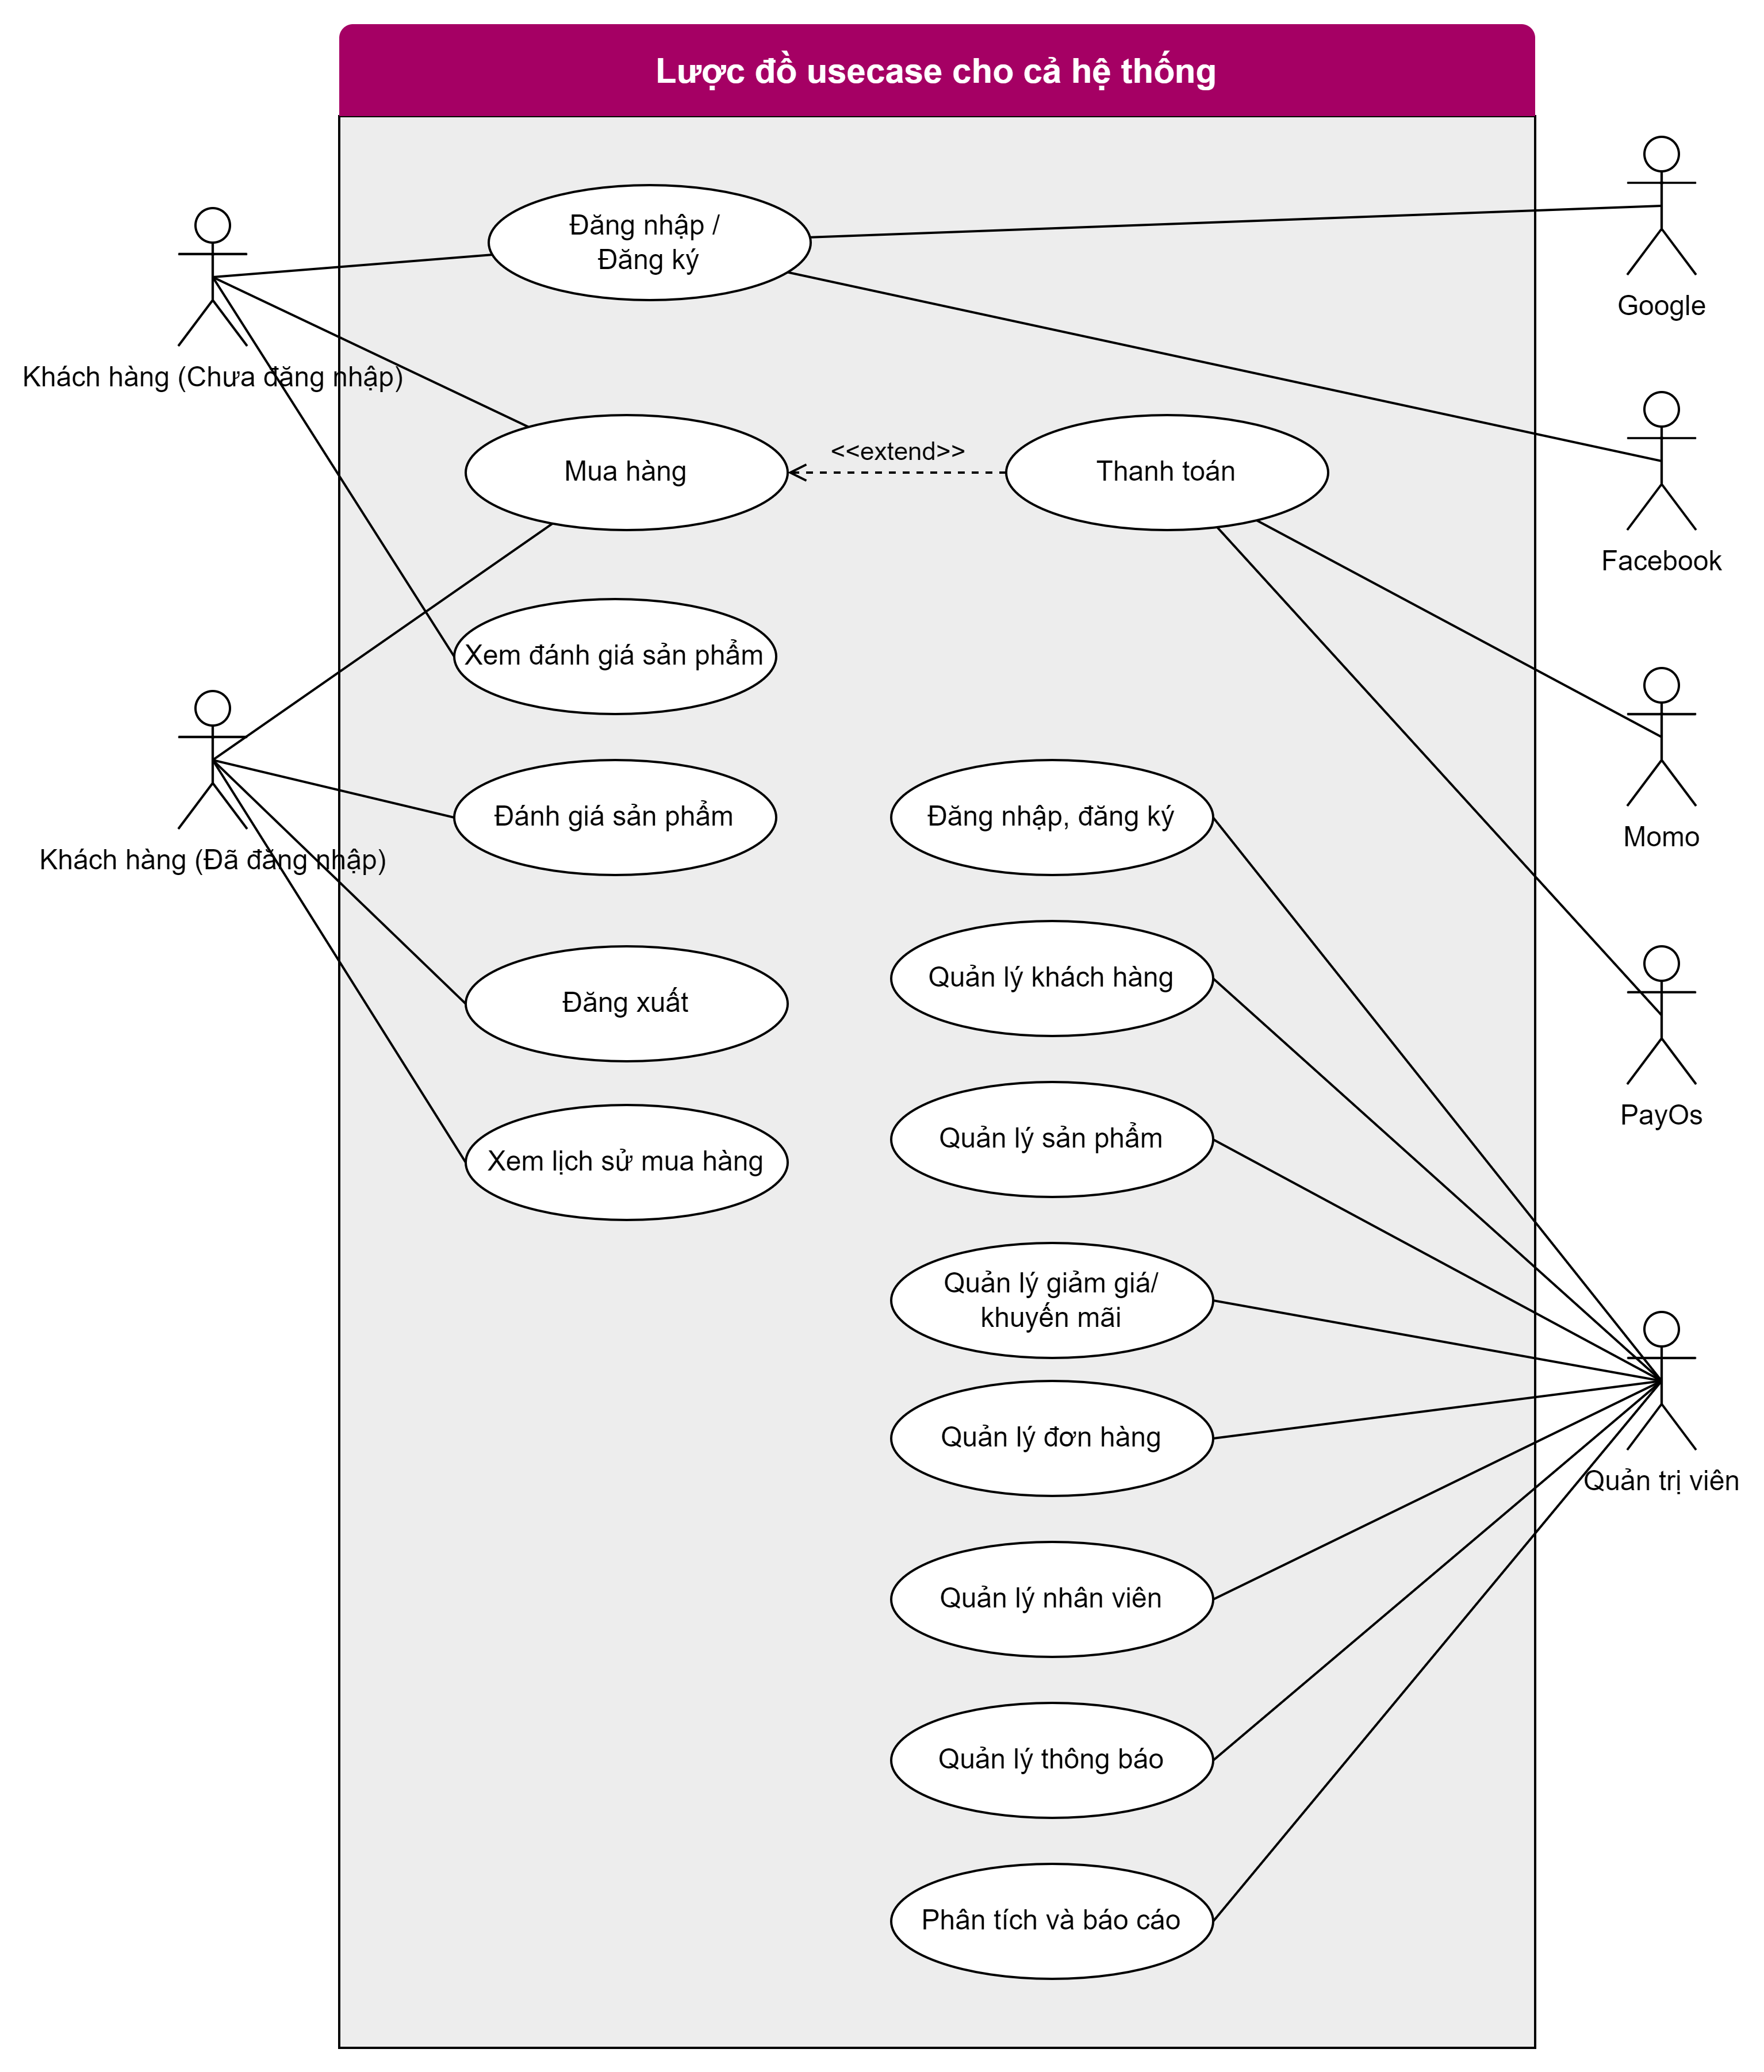
\includegraphics[width=14cm]{Images/usecase/OverallUsecase.png}
    \newline
    \caption{Sơ đồ Use-Case cho toàn bộ hệ thống}
    \label{fig:enter-label}
\end{figure}

\newpage
\subsection{Sơ đồ usecase chi tiết}
\subsubsection{Đăng nhập, đăng ký}
\begin{enumerate}[a.]
    \item \textbf{Use-case diagram}
        \begin{figure}[H]
            \centering
            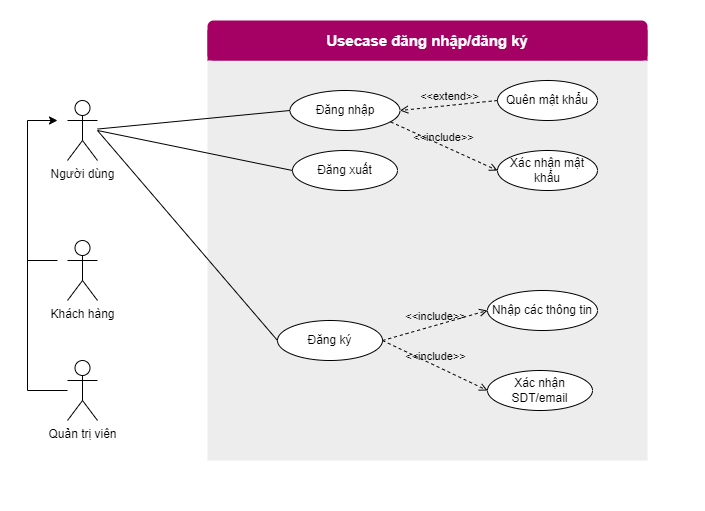
\includegraphics[width=15cm]{Images/usecase/Login-usecase.png}
            \caption{Use case diagram cho đăng nhập và đăng ký}
        \end{figure}
        
    \begin{longtable}{|p{3.5cm}|p{11.5cm}|}
        \hline
        Name &
          Đăng nhập \\ \hline
        Actor(s) &
          Người dùng \\ \hline
        Description &
          Cho phép người dùng đăng nhập vào hệ thống \\ \hline
        Trigger &
          Người dùng chọn nút "Đăng nhập" tại trang giao diện chính của hệ thống\\ \hline
        Pre-condition(s) & \begin{tabular}{@{}p{\linewidth}}
            - Người dùng chưa đăng nhập vào hệ thống\\
            - Người dùng có tài khoản để đăng nhập\\
            - Thiết bị của người dùng phải có kết nối internet ổn định
        \end{tabular} \\ 
          \hline
        Post-condition(s) & Người dùng đăng nhập thành công vào hệ thống.\\ 
        \hline
        Main Flow &
          \begin{tabular}[c]{@{}p{\linewidth}}
            1. Người dùng chọn "Đăng nhập" \\
            2. Hệ thống chuyển đến trang đăng nhập \\
            3. Người dùng nhập số điện thoại/email và mật khẩu \\
            4. Người dùng nhấn nút "Đăng nhập" \\
            5. Hệ thống kiểm tra số điện thoại/email và mật khẩu \\
            6. Hệ thống cập nhật lại giao diện người dùng tùy theo thông tin tài khoản.
        \end{tabular} \\ 
        \hline
        Alternative Flow &
        \begin{tabular}[c]{@{}p{\linewidth}} 
          \textbf{A1: Tại bước 2.}\\
           2.1: Người dùng nhấn vào "Quên mật khẩu" \\
           2.2: Hệ thống cung cấp phương pháp đặt lại mật khẩu của tài khoản\\
        Tiếp tục bước 3 trong Main Flow \\
            \textbf{A2: Tại bước 2.} \\
            2.1. Người dùng nhấn vào "Đăng ký tài khoản"\\
            2.2. Hệ thống chuyển đến trang đăng ký tài khoản \\
        Tiếp tục bước 2 trong Main Flow\\
        \end{tabular} \\ 
        \hline
        Exception & 
        \begin{tabular}[c]{@{}p{\linewidth}} 
          \textbf{E1: Tại bước 5.}\\
           5.1: Người dùng nhập sai số điện thoại/email hoặc mật khẩu\\
           5.2:  Hệ thống hiển thị thông tin đăng nhập sai \\
          Quay lại bước 2 trong Main Flow.\\
        \end{tabular} \\ \hline
        \caption{Use-case đăng nhập}
    \end{longtable}
    
    \newpage
    
    \begin{longtable}{|p{3.5cm}|p{11.5cm}|}
        \hline
        Name & Đăng ký \\ 
        \hline
        Actor(s) & Người dùng  \\ 
        \hline
        Description & Cho phép người dùng đăng ký trở thành thành viên \\ 
        \hline
        Trigger & Người dùng chọn "Đăng kí tài khoản" tại trang đăng ký\\ 
        \hline
        Pre-condition(s) & \begin{tabular}[c]{@{}p{\linewidth}}
            - Người dùng có số điện thoại chưa đăng kí tài khoản trên ứng dụng\\
            - Thiết bị của người dùng phải có kết nối internet ổn định
        \end{tabular} \\
        \hline
        Post-condition(s) & Người dùng tạo thành công tài khoản thành viên trên website và đăng nhập thành công vào hệ thống\\ 
        \hline
        Main Flow &
          \begin{tabular}[c]{@{}p{\linewidth}}
            1. Người dùng nhấn vào "Đăng ký tài khoản"\\
            2. Hệ thống chuyển sang giao diện yêu cầu người dùng nhập số điện thoại.\\
            3. Người dùng nhập số điện thoại vào và nhấn "Xác nhận".\\
            4. Hệ thống chuyển sang giao diện yêu cầu người dùng nhập các thông tin bao gồm tên đăng nhập, mật khẩu, xác nhận mật khẩu\\
            5. Người dùng điền đầy đủ thông tin được yêu cầu ở bước 4\\
            6. Người dùng chọn "Đăng ký"\\
            7. Đăng ký thành công và chuyển sang giao diện trang chủ\\
        \end{tabular} \\ 
        \hline
        Alternative Flow &
          \begin{tabular}[c]{@{}p{\linewidth}} 
            \textbf{A1: tại bước 2}\\
            2.1. Nếu người dùng đã có tài khoản, nhấn "Đăng nhập"\\
            2.2. Hệ thống chuyển sang trang đăng nhập\\
            \textbf{A2: tại bước 5}\\
            Người dùng muốn nhập lại số điện thoại khác thì nhấn "Quay lại", tiếp tục bước 2 trong Main Flow\\
        \end{tabular} \\ 
        \hline
        Exception & \begin{tabular}[c]{@{}p{\linewidth}} 
          \textbf{E1: Tại bước 3}\\
            3.1 Số điện thoại người dùng nhập vào không hợp lệ, hệ thống hiển thị thông báo lỗi\\
            Quay lại bước 2 trong Main flow\\
          \textbf{E2: Tại bước 3:}\\
            3.1. Số điện thoại người dùng nhập vào đã được đăng ký trên hệ thống, giao diện hiển thị thông báo "Số điện thoại này đã được đăng ký"\\
            Quay lại bước 2 trong Main Flow\\
            \textbf{E3: tại bước 5}\\
            5.1: Thông tin người dùng nhập vào không hợp lệ, hệ thống hiển thị thông báo lỗi tương ứng và yêu cầu người dùng nhập lại.\\
            Quay lại bước 4 trong Main Flow
        \end{tabular} \\ 
        \hline
        \caption{Use-case đăng ký}
    \end{longtable}
\end{enumerate}

\newpage
\subsubsection{Chức năng đặt hàng sản phẩm}
\begin{enumerate}[a. ]
    \item \textbf{Use-case diagram}
        \begin{figure}[h]
            \centering
            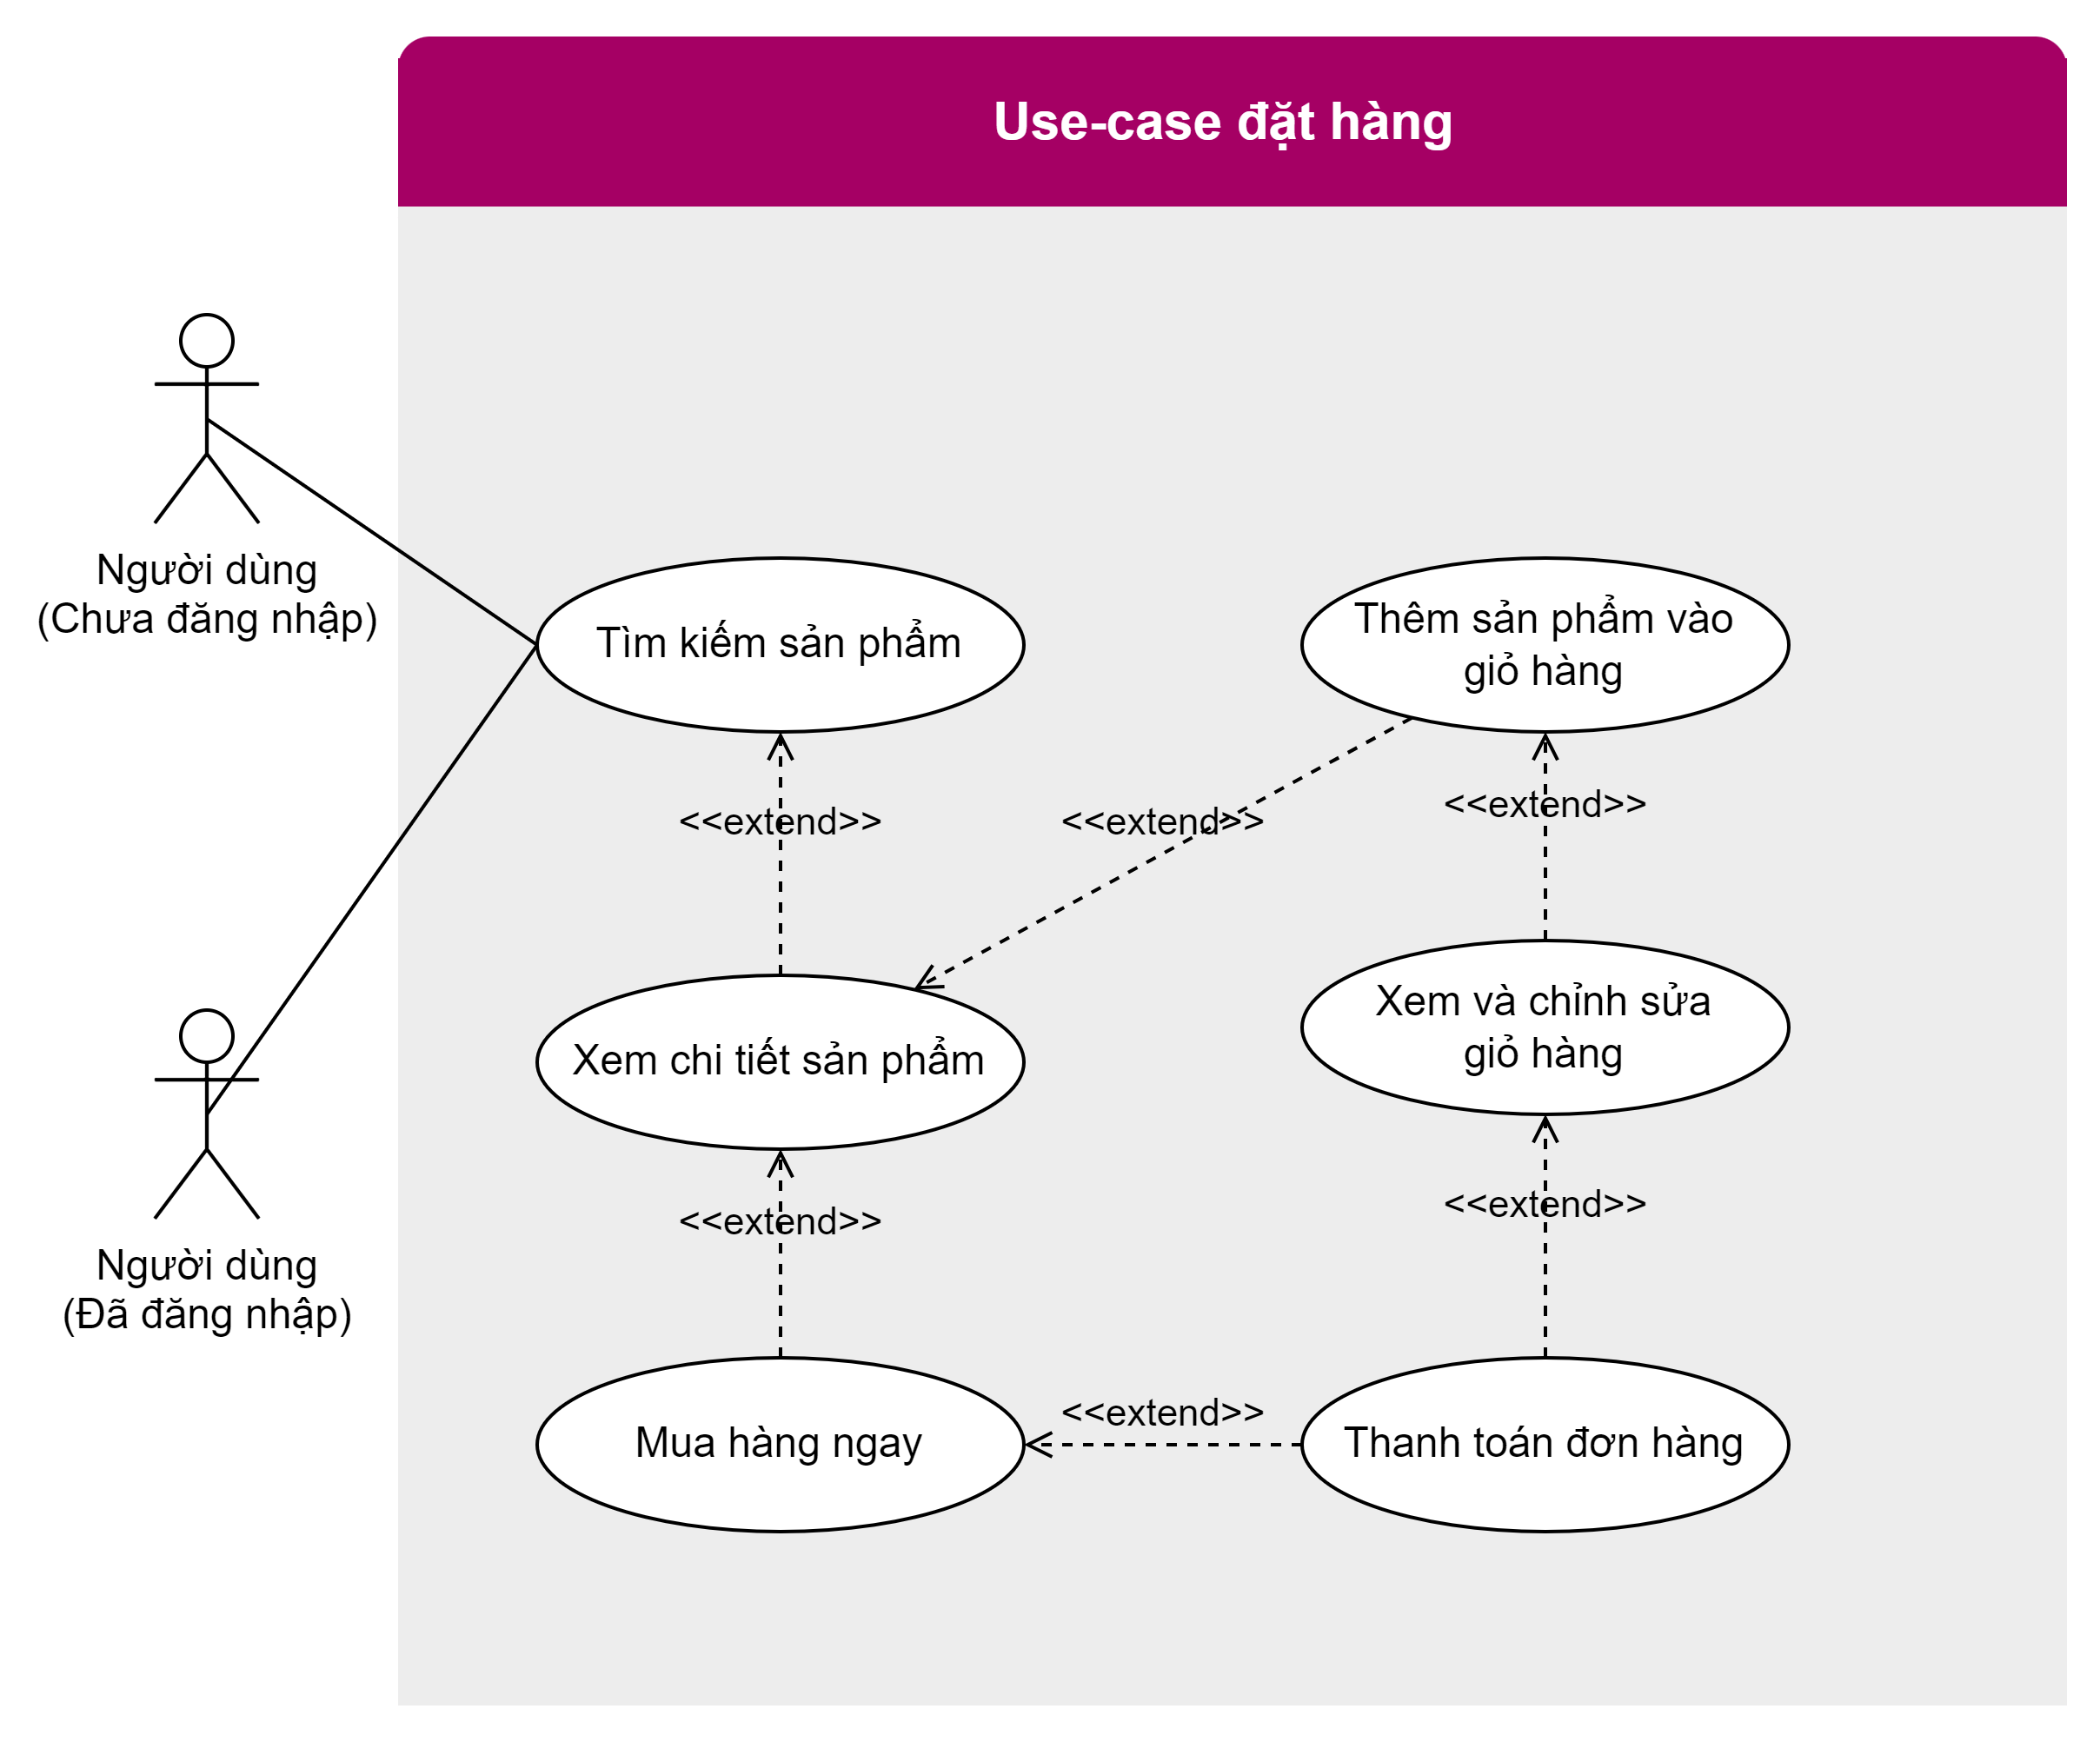
\includegraphics[width=15cm]{Images/usecase/orderUsecase.png}
            \newline
            \caption{Use-case diagram cho đặt hàng sản phẩm}
            \label{fig:enter-label}
        \end{figure}
    \newpage
    
    \item \textbf{Mô tả use-case}
    \begin{longtable}{|p{3.5cm}|p{11.5cm}|}
        \hline
        Name & Tìm kiếm sản phẩm \\ \hline
        Actor(s) &
          Tất cả người dùng \\ \hline
        Description &
          Cho phép người dùng tìm kiếm một mặt hàng cụ thể trên ứng dụng cửa hàng thời trang trực tuyến \\ 
        \hline
        Trigger &
          Người dùng muốn tìm kiếm một sản phẩm nào đó\\ \hline
        Pre-condition(s) & \begin{tabular}[c]{@{}p{\linewidth}}
            - Người dùng phải ở trang chủ của ứng dụng\\
        \end{tabular} \\ 
        \hline
        Post-condition(s) & Người dùng đã tìm được sản phẩm cần mua trong ứng dụng\\ 
        \hline
        Main Flow &
          \begin{tabular}[c]{@{}p{\linewidth}}
            1. Người dùng nhấn vào thanh tìm kiếm trên cùng của ứng dụng \\
            2. Hệ thống chuyển sang giao diện yêu cầu người dùng nhập thông tin cần tìm kiếm\\
            3. Người dùng nhập thông tin tìm kiếm và bấm "OK" ở bàn phím hoặc bấm vào biểu tượng hình kính lúp bên cạnh ô tìm kiếm\\
            4. Hệ thống hiển thị những sản phẩm mà người dùng đã tìm kiếm.
        \end{tabular} \\ 
        \hline
        Alternative Flow &
          \begin{tabular}[c]{@{}p{\linewidth}} 
          \textbf{A1: Tại bước 3.}\\
           3.1. Người dùng bấm "Hủy" trên bàn phím hoặc biểu tượng "x" trên thanh tìm kiếm.\\
           3.2. Hệ thống đưa người dùng về lại trang chủ \\
        \end{tabular} \\ 
        \hline
        Exception & \begin{tabular}[c]{@{}p{\linewidth}} 
          \textbf{ E1: Tại bước 4.}\\
           5.1. Nếu không có sản phẩm được tìm thấy thì hiển thị "Không tìm thấy sản phẩm". \\
          \textbf{ E2: Tại bước 4.}\\
           5.2. Nếu hệ thống có vấn đề thì phải thông báo đến người dùng. \\
        \end{tabular} \\ \hline
    \caption{Use-case tìm kiếm sản phẩm}
    \end{longtable}
    
    \newpage

    \begin{longtable}{|p{3.5cm}|p{11.5cm}|}
        \hline
        Name & Thêm sản phẩm vào giỏ hàng \\ \hline
        Actor(s) &
          Tất cả người dùng \\ \hline
        Description &
          Cho phép người dùng thêm một sản phẩm muốn mua vào giỏ hàng khi người dùng muốn mua nhiều sản phẩm \\ \hline
        Trigger &
          Người dùng muốn mua một sản phẩm nào đó\\ \hline
        Pre-condition(s) & Người dùng phải ở trang thông tin chi tiết của sản phẩm\\
          \hline
        Post-condition(s) & Người dùng đã thêm được sản phẩm cần mua vào trong giỏ hàng\\ \hline
        Main Flow &
          \begin{tabular}[c]{@{}p{\linewidth}}
            1. Người dùng nhấn vào nút "Thêm vào giỏ hàng". \\
            2. Nếu người dùng chưa chọn kích thước hoặc màu sẽ hiển thị lên kích thước và màu để nguời dùng chọn.\\
            3. Sau khi người dùng chọn xong thì bấm "Xác nhận".\\
            4. Hệ thống thêm sản phẩm người dùng chọn vào giỏ hàng.
        \end{tabular} \\ \hline
        Alternative Flow &
          \begin{tabular}[c]{@{}p{\linewidth}} 
          \textbf{A1: Tại bước 3.}\\
           3.1. Người dùng bấm "Hủy" chọn kích thước và màu.\\
           3.2. Hệ thống đưa người dùng về lại trang thông tin sản phẩm \\
        \end{tabular} \\ \hline
          
        Exception & None \\
        \hline
    \caption{Use-case thêm sản phẩm vào giỏ hàng}
    \end{longtable}

    \newpage
    \begin{longtable}{|p{3.5cm}|p{11.5cm}|}
        \hline
        Name & Sửa đổi số lượng sản phẩm trong giỏ hàng \\ \hline
        Actor(s) &
          Tất cả người dùng \\ \hline
        Description &
          Cho phép người dùng thay đổi số lượng sản phẩm muốn mua trong giỏ hàng. \\ \hline
        Trigger &
          Người dùng muốn sửa đổi số lượng sản phẩm trong giỏ hàng.\\ \hline
        Pre-condition(s) & Người dùng phải ở trang giỏ hàng.\\
          \hline
        Post-condition(s) & Người dùng đã sửa số lượng sản phẩm trong giỏ hàng thành công\\ \hline
        Main Flow &
        \begin{tabular}[c]{@{}p{\linewidth}}
            1. Người dùng cần xác định sản phẩm muốn thay đổi số lượng. \\
            2. Người dùng nhấn vào nút "+" để tăng số lượng hoặc "-" để giảm số lượng sản phẩm.\\
            3. Hệ thống tính toán lại giá tiền sản phẩm.\\
        \end{tabular} \\ 
        \hline
        Alternative Flow & None \\
        \hline
        Exception & None \\
        \hline
    \caption{Use-case sửa số lượng sản phẩm trong giỏ hàng}
    \end{longtable}
    
    \newpage
    
    \begin{longtable}{|p{3.5cm}|p{11.5cm}|}
        \hline
        Name & Xóa sản phẩm ra khỏi giỏ hàng \\ \hline
        Actor(s) &
          Tất cả người dùng \\ 
          \hline
        Description &
          Cho phép người dùng xóa một sản phẩm ra khỏi giỏ hàng \\ 
          \hline
        Trigger &
          Người dùng không muốn mua sản phẩm đó nữa và muốn bỏ nó ra giỏ hàng\\ 
          \hline
        Pre-condition(s) & Người dùng phải ở trang giỏ hàng.\\
          \hline
        Post-condition(s) & Người dùng đã xóa sản phẩm ra khỏi giỏ hàng thành công\\ 
        \hline
        Main Flow &
          \begin{tabular}[c]{@{}p{\linewidth}}
            1. Người dùng cần xác định sản phẩm cần xóa ra khỏi giỏ hàng. \\
            2. Người dùng nhấn biểu tượng xóa.\\
            3. Hệ thống hiển thị một thông báo đến người dùng và yêu cầu nhấn vào nút "Xác nhận".\\
            4. Hệ thống xóa sản phẩm ra khỏi giỏ hàng.
        \end{tabular} \\ \hline
        Alternative Flow &
          \begin{tabular}[c]{@{}p{\linewidth}} 
          \textbf{A1: Tại bước 3.}\\
           3.1. Người dùng bấm "Hủy" xóa sản phẩm.\\
           3.2. Hệ thống tắt thông báo. \\
        \end{tabular} \\ \hline
        Exception & None \\
        \hline
    \caption{Use-case xóa sản phẩm ra khỏi giỏ hàng}
    \end{longtable}
    
    \newpage
    \begin{longtable}{|p{3.5cm}|p{11.5cm}|} 
        \hline
        Name & Người dùng muốn đặt mua sản phẩm \\ \hline
        Actor(s) &
          Tất cả người dùng \\ 
          \hline
        Description &
          Cho phép người dùng đặt đơn sản phẩm \\ 
          \hline
        Trigger &
          Người dùng muốn mua sản phẩm\\ 
          \hline
        Pre-condition(s) & \begin{tabular}[c]{@{}p{\linewidth}}
            - Người dùng phải ở trang giỏ hàng và tích vào những sản phẩm cần mua. \\
            - Người dùng đang ở trang chi tiết sản phẩm và bấm "Mua ngay".\\
        \end{tabular} \\ 
        \hline
        Post-condition(s) & Người dùng đã đặt hàng thành công và chuyển sang phương thức thanh toán\\ 
        \hline
        Main Flow &
          \begin{tabular}[c]{@{}p{\linewidth}}
            1. Người dùng cần xác định sản phẩm cần mua ở trong giỏ hàng hoặc ở trang chi tiết sản phẩm cần mua . \\
            2. Người dùng nhấn nút "Mua ngay".\\
            3. Hệ thống đưa người dùng đến trang xác nhận đơn hàng.\\
            4. Người dùng xác nhận địa chỉ nhận hàng.\\
            5. Người dùng nhập hoặc áp mã giảm giá (nếu có).\\
            6. Hệ thống kiểm tra mã giảm giá có hợp lệ.\\
            7. Hệ thống tính tổng tiền cho đơn hàng.
        \end{tabular} \\ \hline
        Alternative Flow &
          \begin{tabular}[c]{@{}p{\linewidth}} 
          \textbf{A1: Tại bước 4: Người dùng chưa đăng nhập}\\
           4.1. Người dùng điền tên, số điện thoại và địa chỉ.\\
           4.2. Tiếp tục bước 5. \\
        \end{tabular} \\ \hline
        Exception & None \\
        \hline
        \caption{Use-case đặt hàng}
    \end{longtable}
\end{enumerate}
\newpage

\subsubsection{Phương thức thanh toán}
\begin{enumerate}[a. ]
    \item \textbf{Use-case Diagram}
        \begin{figure}[h]
            \centering
            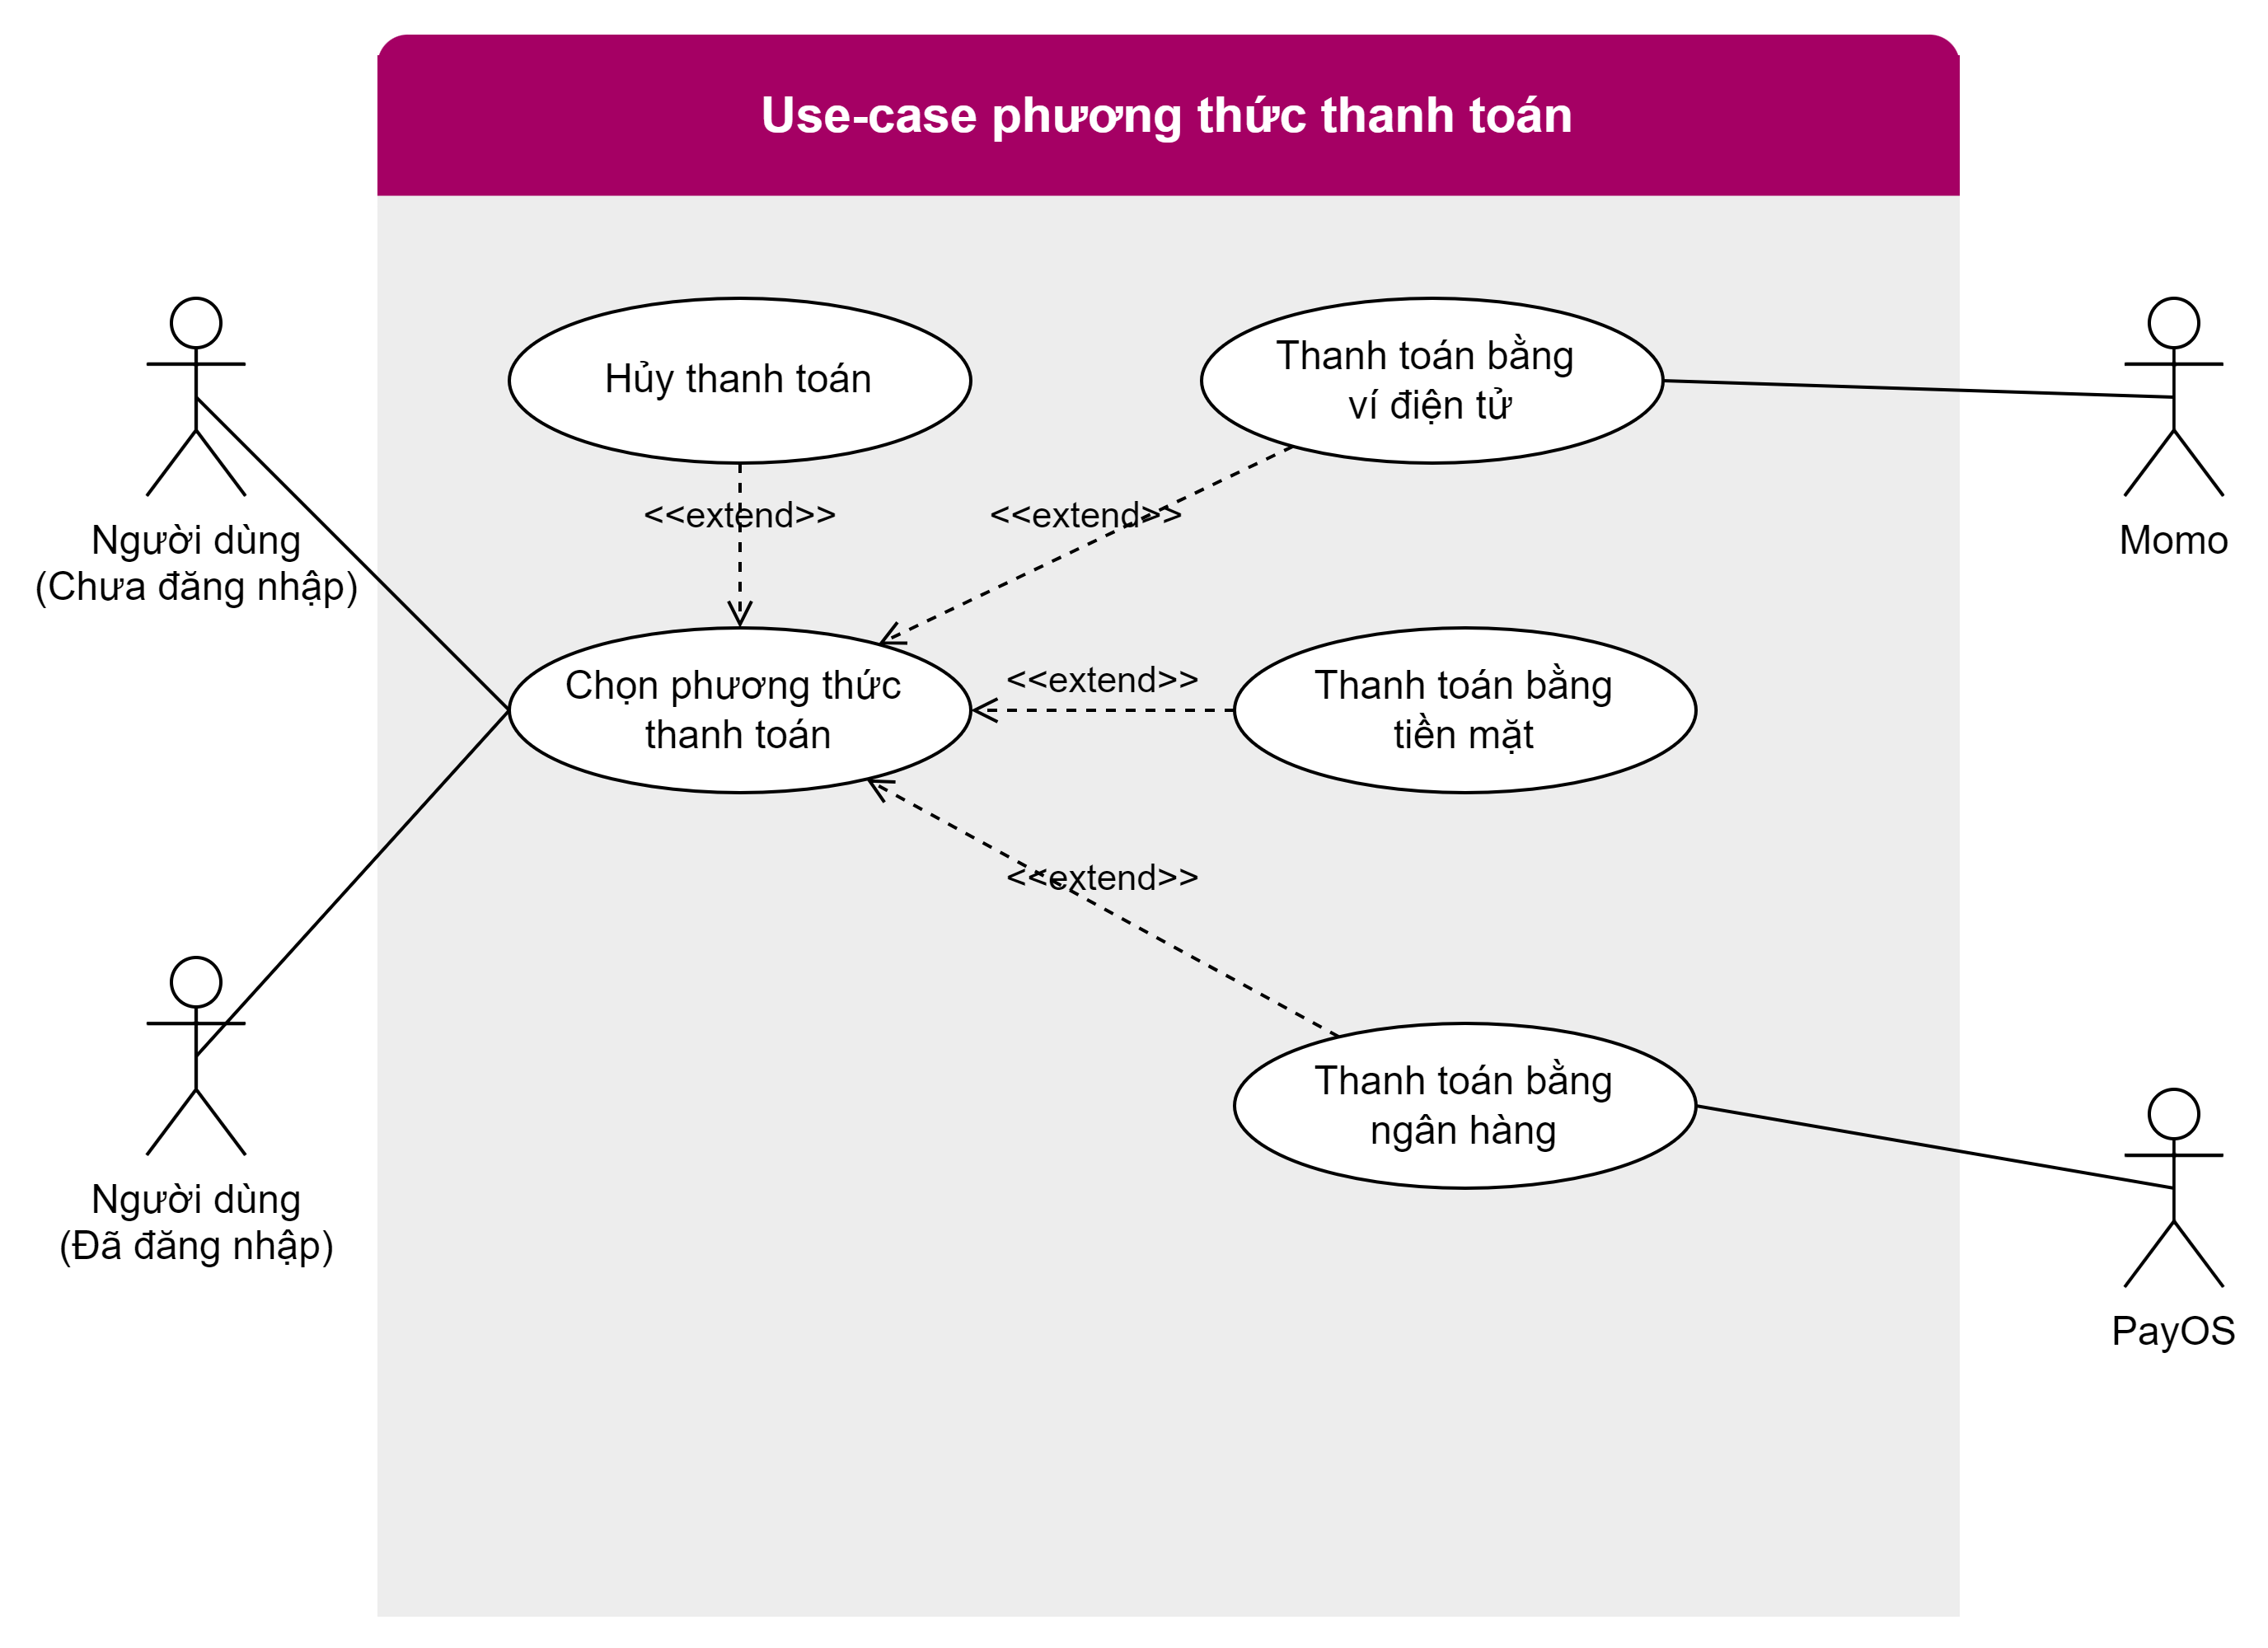
\includegraphics[width=15cm]{Images//usecase/UseCasePaymentMomo.png}
            \newline
            \caption{Use-case diagram cho phương thức thanh toán}
            \label{fig:enter-label}
        \end{figure}
    \newpage
    \item \textbf{Mô tả use-case}
    
    \begin{longtable}{|p{3.5cm}|p{11.5cm}|}  
        \hline
        Name & Thanh toán bằng ví Momo \\ \hline
        Actor(s) &
          Tất cả người dùng \\ 
          \hline
        Description &
          Cho phép người dùng thanh toán đơn hàng bằng ví điện tử \\ 
          \hline
        Trigger &
          Người dùng muốn mua thanh toán sản phẩm bằng Momo\\ 
          \hline
        Pre-condition(s) & \begin{tabular}[c]{@{}p{\linewidth}}
            - Người dùng phải ở trang chọn phương thức thanh toán. \\
            - Người dùng phải có và cài đặt ứng dụng Momo.\\
        \end{tabular} \\ 
        \hline
        Post-condition(s) & Người dùng thanh toán thành công đơn hàng\\ 
        \hline
        Main Flow &
          \begin{tabular}[c]{@{}p{\linewidth}}
            1. Người dùng chọn phương thức thanh toán Momo . \\
            2. Người dùng nhấn nút "Điều hướng sang ứng dụng Momo".\\
            3. Hệ thống đưa người dùng đến ứng dụng Momo.\\
            4. Người dùng thực hiện chuyển tiền.\\
            5. Ứng dụng Momo chuyển về lại ứng dụng cửa hàng.\\
            6. Hệ thống hiển thị thông tin đơn hàng được thanh toán thành công.\\
        \end{tabular} \\ \hline
        Alternative Flow &
          \begin{tabular}[c]{@{}p{\linewidth}} 
          \textbf{A1: Tại bước 2: Người dùng thực hiện thanh toán bằng mã QR}\\
           2.1. Người dùng quét mã thanh toán bằng điện thoại khác hoặc lưu mã QR.\\
           2.2. Hệ thống kiểm tra đơn hàng đã được thanh toán chưa. \\
           2.3. Tiếp tục bước 6.
        \end{tabular} \\ \hline
        Exception & \begin{tabular}[c]{@{}p{\linewidth}}
            \textbf{E1: Tại bước 2: người dùng không có ứng dụng Momo}\\
            Không thể chuyển sang ứng dụng Momo được.
        \end{tabular}\\ 
        \hline
        \caption{Use-case thanh toán ví điện tử}
    \end{longtable}
    
    \newpage
    \begin{longtable}{|p{3.5cm}|p{11.5cm}|}
        \hline
        Name & Thanh toán bằng ngân hàng \\ \hline
        Actor(s) &
          Người dùng \\ \hline
        Description &
          Cho phép người dùng thanh toán đơn hàng bằng tài khoản ngân hàng. \\ \hline
        Trigger &
          Người dùng muốn thanh toán đơn hàng bằng tài khoản ngân hàng\\ \hline
        Pre-condition(s) & Người dùng phải ở trang chọn phương thức thanh toán.\\
          \hline
        Post-condition(s) & Người dùng thanh toán đơn hàng thành công.\\ \hline
        Main Flow &
        \begin{tabular}[c]{@{}p{\linewidth}}
           1. Người dùng chọn phương thức thanh toán bằng ngân hàng . \\
            2. Hệ thống điều hướng người dùng sang trình duyệt.\\
            3. Người dùng thực hiện quét mã QR để thanh toán.\\
            4. Hệ thống thứ 3 kiểm tra giao dịch thành công sẽ đẩy ngược về lại ứng dụng bán hàng.\\
            5. Hệ thống hiển thị thông tin đơn hàng được thanh toán thành công.\\
        \end{tabular} \\ 
        \hline
        Alternative Flow & None \\
        \hline
        Exception & None \\ 
        \hline
    \caption{Use-case thanh toán bằng ngân hàng}
    \end{longtable}
\end{enumerate}

\newpage

\subsubsection{Quản lý thông tin cá nhân}
\begin{enumerate}[a. ]
    \item \textbf{Use-case Diagram}
        \begin{figure}[H]
            \centering
            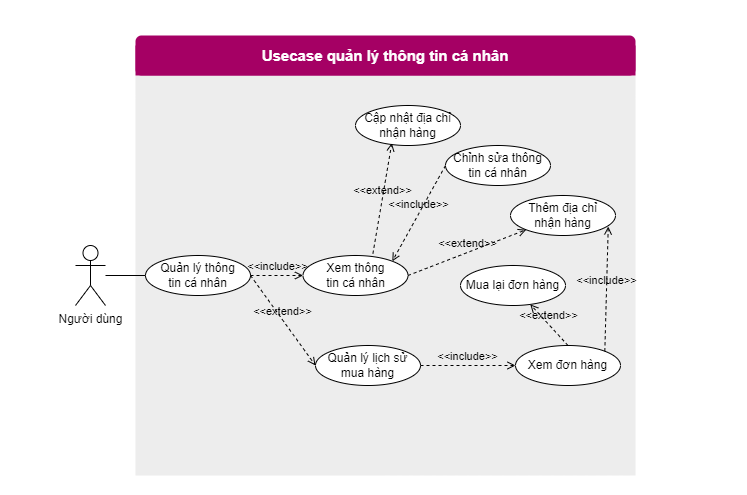
\includegraphics[width=17cm]{Images/usecase/ManageProfile.png}
            \newline
            \caption{Use-case diagram cho quản lý thông tin cá nhân}
        \end{figure}
    \newpage
    \item \textbf{Mô tả use-case}
    \begin{longtable}{|p{3.5cm}|p{11.5cm}|}
        \hline
        Name & Quản lý thông tin cá nhân \\ \hline
        Actor(s) &
          Người dùng \\ \hline
        Description &
          Cho phép người dùng xem, thay đổi thông tin cá nhân, xem lịch sử đơn hàng, thêm và cập nhật địa chỉ nhận hàng \\ \hline
        Trigger &
          Người dùng nhấn vào "Tài khoản của tôi"\\ \hline
        Pre-condition(s) & Người dùng đã đăng nhập tài khoản thành công.\\
          \hline
        Post-condition(s) & Người dùng thấy được thông tin cá nhân thành công\\ \hline
        Main Flow &
        \begin{tabular}[c]{@{}p{\linewidth}}
            1. Người dùng nhấn vào "Tài khoản của tôi" \\
            2. Hệ thống hiển thị thông tin cá nhân của người dùng\\
            3. Người dùng xem toàn bộ thông tin cá nhân\\
        \end{tabular} \\ 
        \hline
         Alternative Flow &
          \begin{tabular}[c]{@{}p{\linewidth}} 
          \textbf{A1: Tại bước 3.}\\
                  3.1: Người dùng chỉnh sửa thông tin cá nhân\\
        3.2: Hệ thống hiển thị màn hình để chỉnh sửa thông tin cá nhân\\
        3.3: Người dùng chỉnh sửa các thông tin cá nhân\\
        3.4 Người dùng nhấn cập nhật để thoát khỏi giao diện chỉnh sửa thông tin cá nhân. Hệ thống xác nhận chỉnh sửa thông tin cá nhân thành công.\\
\textbf{A2: Tại bước 3.}\\
        3.1: Người dùng nhấn vào nút "Xem lịch sử đơn hàng"\\
        3.2: Hệ thống hiển thị tất cả các đơn hàng đã mua\\

        \end{tabular} \\ \hline
        Exception & None \\
        \hline
    \caption{Use-case quản lý thông tin cá nhân}
    \end{longtable}
    
\end{enumerate}
\newpage
\subsubsection{Quản lý nhân viên}
\begin{enumerate}[a.]
    \item \textbf{Use-case diagram}
        \begin{figure}[H]
            \centering
            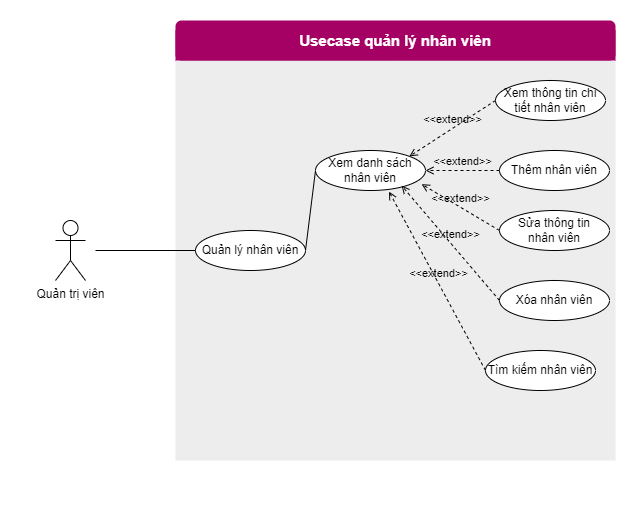
\includegraphics[width=16cm]{Images/usecase/ManageEmployee.png}
            \caption{Use case diagram cho quản lý nhân viên}
        \end{figure}
        
    \newpage
    \item \textbf{Mô tả usecase}
    \begin{longtable}{|p{3.5cm}|p{11.5cm}|}
        \hline
        Name &
          Xem thông tin chi tiết của nhân viên \\ \hline
        Actor(s) &
          Quản trị viên \\ \hline
        Description &
          Cho phép quản trị viên xem thông tin chi tiết của tất cả các nhân viên trên hệ thống \\ \hline
        Trigger &
          Quản trị viên chọn nút "Quản lý nhân viên" tại trang giao diện chính của hệ thống\\ \hline
        Pre-condition(s) & \begin{tabular}[c]{@{}p{\linewidth}}
- Quản trị viên đã đăng nhập vào hệ thống bằng tài khoản Manager\\
        \end{tabular} \\ 
          \hline
        Post-condition(s) &Quản trị viên xem được danh sách tất cả các nhân viên trong hệ thống.\\ \hline
        
        Main Flow &
          \begin{tabular}[c]{@{}p{\linewidth}}
            1 . Hệ thống hiển thị danh sách tất cả các nhân viên\\
        2 . Quản trị viên chọn cụ thể một nhân viên bằng cách nhấn vào nút icon xem chi tiết\\
        3 . Hệ thống hiển thị thông tin chi tiết của nhân viên\\
        \end{tabular} \\ 
        \hline
        Alternative Flow & \begin{tabular}[c]{@{}p{\linewidth}} 
            \textbf{A1: Tại bước 1: }\\
            1.1. Quản trị viên nhấn tìm kiếm tên 1 nhân viên cụ thể\\
            1.2.Hệ thống trả về các nhân viên thỏa mãn tiêu chí tìm kiếm \\
        \end{tabular} \\ 
        \hline
        Exception & None \\
        \hline
        \caption{Use-case xem thông tin chi tiết của nhân viên}
    \end{longtable}
    \newpage
    
    \begin{longtable}{|p{3.5cm}|p{11.5cm}|}        
        \hline
        Name &  Thêm nhân viên mới \\ \hline
        Actor(s) &
          Quản trị viên \\ \hline
        Description &
          Cho phép quản trị viên thêm một nhân viên mới\\ \hline
        Trigger &
          Quản trị viên nhấn vào thêm nhân viên\\ \hline
        Pre-condition(s) &
          \begin{tabular}[c]{@{}p{\linewidth}}
        Quản trị viên đã đăng nhập vào tài khoản của mình\\
        Quản trị viên đang trong màn hình quản lý nhân viên\\
        \end{tabular} \\ \hline
        Post-condition(s) & Quản trị viên thêm nhân viên thành công\\ \hline
        Main Flow &
          \begin{tabular}[c]{@{}p{\linewidth}}
        1 . Hệ thống chuyển sang giao diện nhập thông tin cho nhân viên mới\\
        2 . Quản trị viên nhập lần lượt các thông tin mà hệ thống yêu cầu (tên nhân viên, ngày sinh, địa chỉ, giới tính,...)\\
        3 . Quản trị viên nhấn "Xác nhận" để thoát khỏi giao diện thêm nhân viên\\
        4 . Hệ thống xác nhận thêm nhân viên thành công\\
        \end{tabular} \\ \hline
        Alternative Flow &
          None \\ \hline
        Exception & \begin{tabular}[c]{@{}p{\linewidth}} 
        \textbf{E1: Tại bước 3:}\\
        - Hệ thống hiển thị lỗi "Tên/địa chỉ/... không hợp lệ"\\
        - Hệ thống hiển thị lỗi "Không được để trống thông tin"\\
        \end{tabular} \\ \hline
        \caption{Use-case thêm nhân viên}
    \end{longtable}
    \newpage
    \begin{longtable}{|p{3.5cm}|p{11.5cm}|}
        \hline
        Name & Tìm kiếm nhân viên\\ \hline
        Actor(s) &
          Quản trị viên \\ \hline
        Description &
          Cho phép quản trị viên tìm kiếm nhân viên\\ \hline
        Trigger &
          \begin{tabular}[c]{@{}p{\linewidth}} 
        Quản trị viên nhấn vào ô tìm kiếm nhân viên\\
        
        \end{tabular} \\ \hline
        Pre-condition(s) & \begin{tabular}[c]{@{}p{\linewidth}} 
        Quản trị viên đã đăng nhập vào tài khoản của mình\\
        Quản trị viên đang trong màn hình quản lý nhân viên\\
        \end{tabular}\\
          \hline
        Post-condition(s) & Quản trị viên xem được thông tin nhân viên đã tìm kiếm\\ \hline
        Main Flow &
          \begin{tabular}[c]{@{}p{\linewidth}}
        1 . Quản trị viên nhập từ khóa tên của nhân viên cần tìm, rồi nhấn tìm kiếm\\
        2 . Hệ thống trả về danh sách tất cả nhân viên thỏa mãn yêu cầu của từ khóa \\
        \end{tabular} \\ \hline
        Alternative Flow & None
         \\ \hline
        Exception & \begin{tabular}[c]{@{}p{\linewidth}} 
        \textbf{E1: Tại bước 2:}\\
        - Hệ thống hiển thị lỗi "Không có nhân viên thỏa mãn yêu cầu"\\
        \end{tabular} \\ \hline
        \caption{Use-case tìm kiếm nhân viên}
    \end{longtable}
    \newpage
    \begin{longtable}{|p{3.5cm}|p{11.5cm}|}        
        \hline
        Name & Chỉnh sửa thông tin nhân viên\\ \hline
        Actor(s) &
          Quản trị viên \\ \hline
        Description &
          Cho phép quản trị viên thay đổi thông tin nhân viên trên hệ thống\\ \hline
        Trigger &
          Quản trị viên nhấn vào "Thay đổi thông tin nhân viên" \\ \hline
        Pre-condition(s) & \begin{tabular}[c]{@{}p{\linewidth}} 
        Quản trị viên đã đăng nhập vào tài khoản của mình\\
        Quản trị viên đang trong màn hình quản lý nhân viên\\
        Quản trị viên đã chọn được nhân viên cần thay đổi thông tin\\
        \end{tabular}\\
        \hline
        Post-condition(s) & Quản trị viên đã thay đổi thông tin thành công cho nhân viên\\ \hline
        Main Flow &
          \begin{tabular}[c]{@{}p{\linewidth}}
        1 . Hệ thống hiển thị 1 màn hình để chỉnh sửa các thông tin cần cho nhân viên\\
        2 . Quản trị viên chỉnh sửa lần lượt các thông tin của nhân viên\\
        3 . Quản trị viên nhấn "Cập nhật" để thoát khỏi giao diện chỉnh sửa thông tin nhân viên\\
        4 . Hệ thống xác nhận chỉnh sửa thông tin nhân viên thành công\\
        \end{tabular} \\ \hline
        Alternative Flow &
          None \\ \hline
        Exception & None \\ \hline
        \caption{Use-case chỉnh sửa thông tin nhân viên}
    \end{longtable}
    \newpage
    \begin{longtable}{|p{3.5cm}|p{11.5cm}|}
        \hline
        Name & Xóa nhân viên\\ \hline
        Actor(s) &
         Quản trị viên\\ \hline
        Description &
          Cho phép quản trị viên xóa nhân viên khỏi hệ thống\\ \hline
        Trigger &
          Quản trị viên nhấn vào "Xóa nhân viên" \\ \hline
        Pre-condition(s) & \begin{tabular}[c]{@{}p{\linewidth}} 
        Quản trị viên đã đăng nhập vào tài khoản của mình\\
        Quản trị viên đang trong màn hình quản lý nhân viên\\
        Quản trị viên đã chọn được nhân viên muốn xóa\\   
        \end{tabular}\\
        \hline
        Post-condition(s) & Quản trị viên xóa thành công nhân viên khỏi hệ thống\\ \hline
        Main Flow &
          \begin{tabular}[c]{@{}p{\linewidth}}
        1 . Hệ thống hiển thị 1 cảnh báo yêu cầu xác nhận xóa nhân viên\\
        2 . Quản trị viên nhấn "Xác nhận xóa"\\
        3 . Hệ thống xác nhận xóa nhân viên thành công\\
        4 . Quản trị viên nhấn "Xác nhận" để thoát khỏi giao diện xóa nhân viên và trở về giao diện quản lý nhân viên
        \\
        \end{tabular} \\ \hline
        Alternative Flow & None\\ \hline 
        Exception & None \\ \hline
        \caption{Use-case xóa nhân viên}
    \end{longtable}
\end{enumerate}
\newpage
\subsubsection{Đánh giá và nhận xét}
\begin{enumerate}[a. ]
    \item \textbf{Use-case diagram}
        \begin{figure}[h]
            \centering
            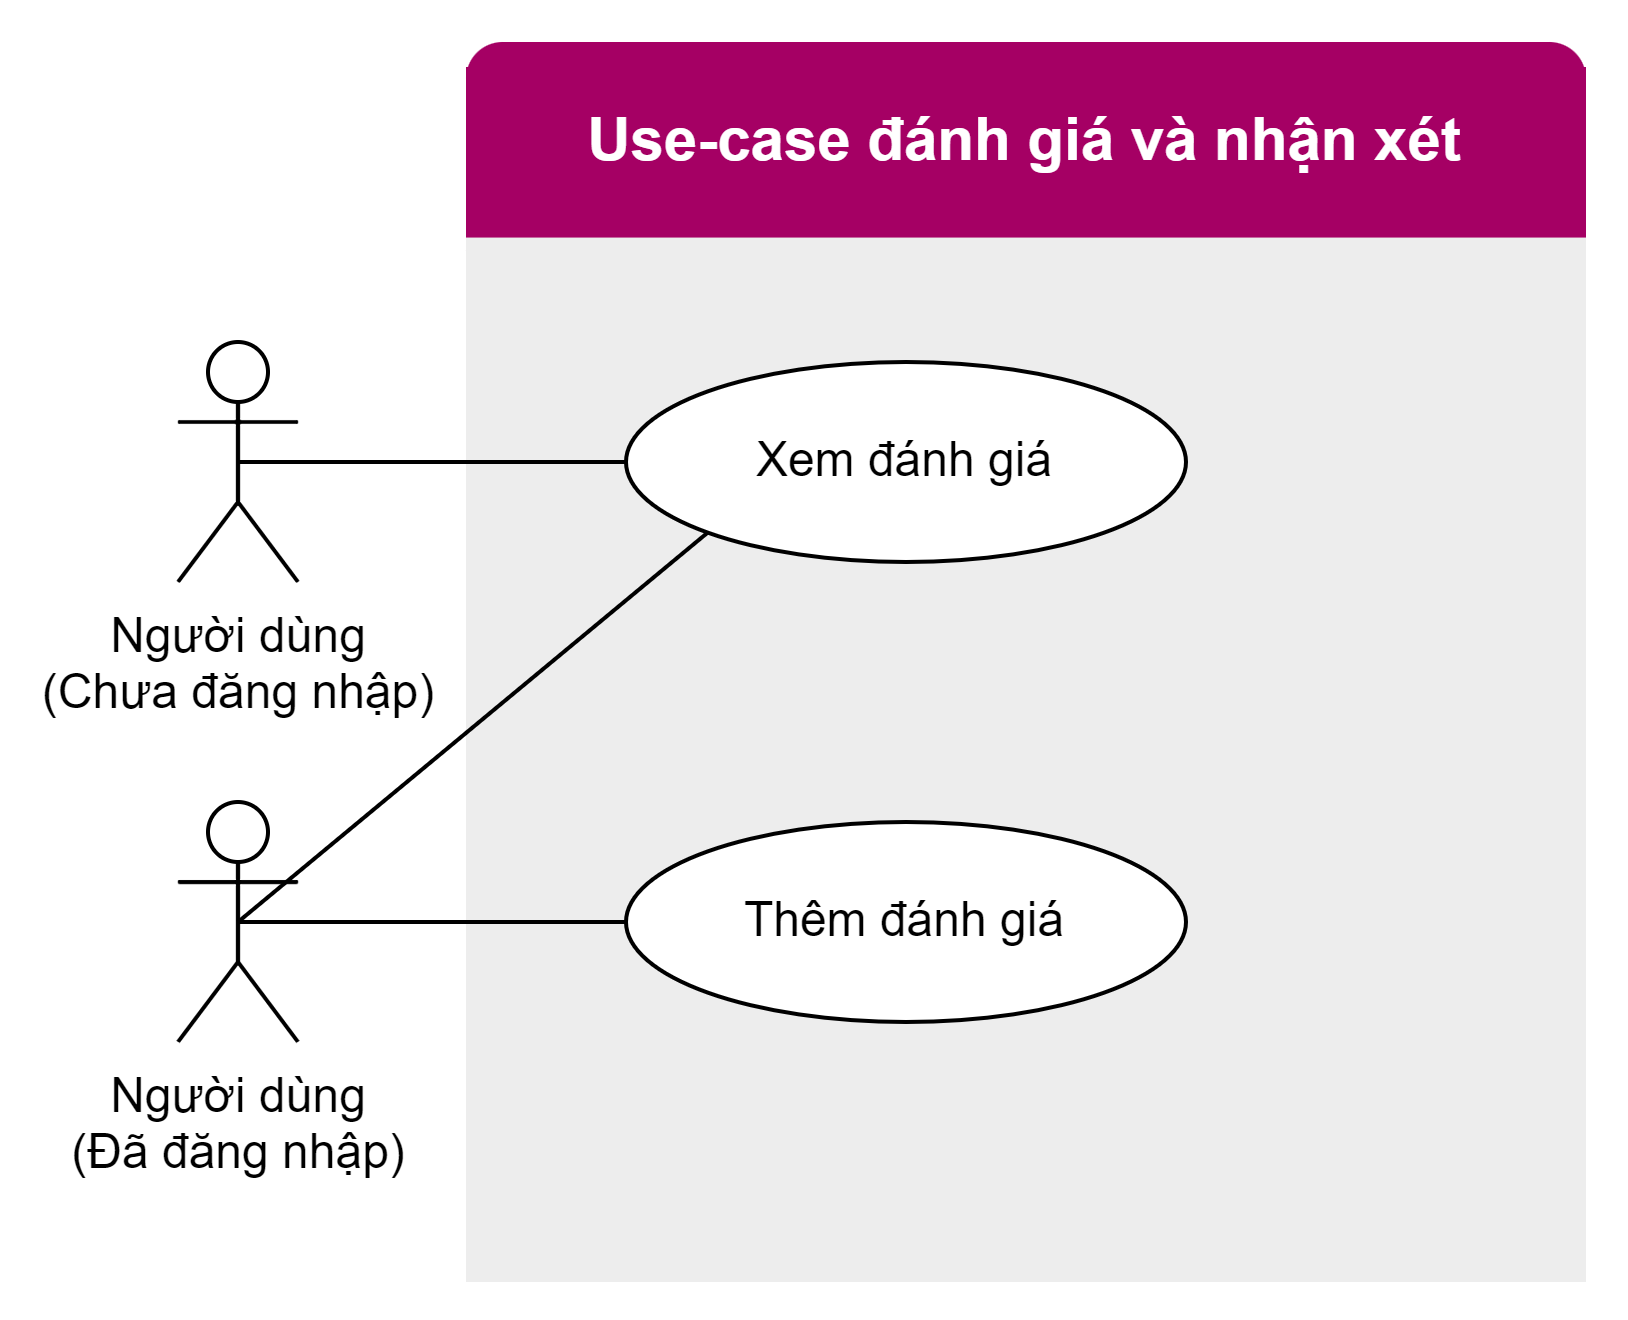
\includegraphics[width=10cm]{Images//usecase/use-case-nx.png}
            \newline
            \caption{Use-case diagram cho đánh giá và nhận xét}
            \label{fig:enter-label}
        \end{figure}
\end{enumerate}


\newpage
\subsubsection{Quản lý giảm giá (quản trị viên)}
\begin{enumerate}[a.]
    \item \textbf{ Use-case diagram}
    \begin{figure}[H]
            \centering
            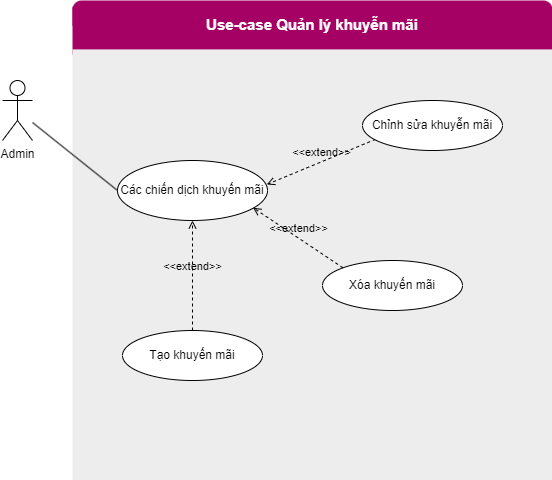
\includegraphics[width=10cm]{Images/usecase/Usecase_khuyenMai.drawio.png}
            \newline
            \caption{Use-case diagram cho quản lý khuyến mãi}
        \end{figure}
        \newpage
    \item \textbf{Mô tả use-case}
    \begin{enumerate}[]
    
        \begin{longtable}{|p{3.5cm}|p{11.5cm}|}
        \hline
        Name & Quản trị viên tạo mới một mã giảm giá \\ \hline
        Actor(s) &
          Quản trị viên \\ 
          \hline
        Description &
          Cho phép quản trị viên tạo mã giảm giá \\ 
          \hline
        Trigger &
          Quản trị viên muốn tạo mới một sự kiện giảm giá\\ 
          \hline
        Pre-condition(s) & \begin{tabular}[c]{@{}p{\linewidth}}
            Quản trị viên đang ở trang quản lý mã giảm giá và tích chọn tạo mới mã giảm giá. \\
        \end{tabular} \\ 
        \hline
        Post-condition(s) & Quản trị viên tạo mới thành công một mã giảm giá mới\\ 
        \hline
        Main Flow &
          \begin{tabular}[c]{@{}p{\linewidth}}
            1. Quản trị viên chọn tạo mới mã giảm giá cho toàn bộ khách hàng. \\
            2. Quản trị viên điền thống tin về chiến dịch khuyến mãi như tên, mô tả, khuyến mãi theo phần trăm (\%) hay giá tiền cố định, thời hạn; chọn tầm vực khách hàng hưởng khuyến mãi đó.\\
            3. Quản trị viên chọn lưu thay đổi.\\
            4. Hệ thống thoát ra khỏi màn hình tạo mới và đưa quản trị viên về lại trang quản lý khuyến mại và thêm mới chiến dịch khuyến mãi quản trị viên vừa tạo.
        \end{tabular} \\ \hline
        Alternative Flow &
          \begin{tabular}[c]{@{}p{\linewidth}} 
          \textbf{A1: Tại bước 2.}\\
           2.1. Quản trị viên bấm "Hủy" tạo mới.\\
           2.2. Hệ thống đưa quản trị viên về lại trang quản lý khuyến mãi. \\
        \end{tabular} \\ \hline
        Exception & None \\
        \hline
        \caption{Use-case tạo mới một khuyến mãi}
        \end{longtable}
        
        \newpage
        
    \begin{longtable}{|p{3.5cm}|p{11.5cm}|}
        \hline
        Name & Quản trị viên chỉnh sửa mã giảm giá \\ \hline
        Actor(s) &
          Quản trị viên \\ 
          \hline
        Description &
          Cho phép quản trị viên chỉnh sửa mã giảm giá \\ 
          \hline
        Trigger &
          Quản trị viên muốn chỉnh sửa sự kiện giảm giá\\ 
          \hline
        Pre-condition(s) & \begin{tabular}[c]{@{}p{\linewidth}}
            Quản trị viên đang ở trang quản lý chiến dịch giảm giá". \\
        \end{tabular} \\ 
        \hline
        Post-condition(s) & Quản trị viên chỉnh sửa thành công một mã giảm giá\\ 
        \hline
        Main Flow &
          \begin{tabular}[c]{@{}p{\linewidth}}
            1. Quản trị viên cần xác định chiến dịch nào cần thay đổi\\
            2. Quản trị viên nhấn vào biểu tượng chỉnh sửa của chiến dịch khuyến mãi mà admin muốn chỉnh sửa.\\
            3. Hệ thống chuyển quản trị viên vào màn hỉnh để chỉnh sửa thống tin của chiến dịch.\\
            4. Quản trị viên chọn lưu thay đổi.\\
            5. Hệ thống chuyển về màn hình quản lý khuyến mãi và cập nhật lại thống tin cho chiến dịch khuyến mãi.\\
        \end{tabular} \\ \hline
        Alternative Flow &
          \begin{tabular}[c]{@{}p{\linewidth}} 
          \textbf{A1: Tại bước 3.}\\
           3.1. Quản trị viên bấm "Hủy" chỉnh sửa.\\
           3.2. Hệ thống đưa quản trị viên về lại trang quản lý khuyến mãi. \\
        \end{tabular} \\ \hline
        Exception & None \\
        \hline
        \caption{Use-case chỉnh sửa khuyến mãi}
        \end{longtable}

        \newpage

    \begin{longtable}{|p{3.5cm}|p{11.5cm}|}
        \hline
        Name & Quản trị viên xóa chiến dịch giảm giá \\ \hline
        Actor(s) &
          Quản trị viên \\ 
          \hline
        Description &
          Cho phép quản trị viên xóa chiến dịch giảm giá \\ 
          \hline
        Trigger &
          Quản trị viên muốn xóa sự kiện giảm giá\\ 
          \hline
        Pre-condition(s) & \begin{tabular}[c]{@{}p{\linewidth}}
            Quản trị viên đang ở trang Quản lý mã giảm giá". \\
        \end{tabular} \\ 
        \hline
        Post-condition(s) & Quản trị viên xóa thành công một mã giảm giá\\ 
        \hline
        Main Flow &
          \begin{tabular}[c]{@{}p{\linewidth}}
            1. Quản trị viên cần xác định chiến dịch nào cần thay đổi\\
            2. Quản trị viên nhấn vào biểu tượng xóa của chiến dịch khuyến mãi mà quản trị viên muốn xóa.\\
            3. Hệ thống hiển thị một thống báo đến quản trị viên và yêu cầu nhấn vào nút "Xác nhận".\\
            4. Hệ thống chuyển màn hình sang trang Quản lý khuyến mãi và xóa chiến dịch khuyến mãi.\\
        \end{tabular} \\ \hline
        Alternative Flow &
          \begin{tabular}[c]{@{}p{\linewidth}} 
          \textbf{A1: Tại bước 3.}\\
           3.1. Quản trị viên bấm "Hủy" xóa.\\
           3.2. Hệ thống đưa quản trị viên về lại trang quản lý khuyến mãi. \\
        \end{tabular} \\ \hline
        Exception & None \\
        \hline
        \caption{Use-case xóa khuyến mãi}
        \end{longtable}
    \end{enumerate}
\end{enumerate}

\newpage

% \subsection{Quản lý thông báo (admin)}
% \subsubsection{Đẩy thông báo đến ứng dụng người dùng}
% \subsubsection{Chỉnh sửa thông báo}
% \subsubsection{Xóa thông báo}

\subsubsection{Quản lý khách hàng (quản trị viên)}
\begin{enumerate}[a.]
    \item \textbf{Use-case diagram}
    \begin{figure}[H]
            \centering
            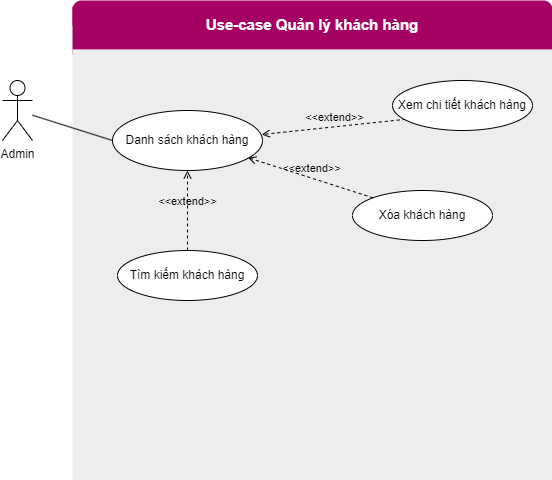
\includegraphics[width=15cm]{Images/usecase/Usecase_quanLyKhachHang.drawio.png}
            \newline
            \caption{Use-case diagram cho quản lý khách hàng}
            \label{figure_customerManagement}
        \end{figure}
    \newpage
    \item \textbf{Mô tả use-case}
    \begin{longtable}{|p{3.5cm}|p{11.5cm}|}
        \hline
        Name &
          Xem thông tin chi tiết của khách hàng \\ \hline
        Actor(s) &
          Quản trị viên \\ \hline
        Description &
          Cho phép quản trị viên xem thông tin chi tiết của tất cả các khách hàng trên hệ thống \\ \hline
        Trigger &
          Quản trị viên chọn nút "Quản lý khách hàng" tại trang giao diện chính của hệ thống\\ \hline
        Pre-condition(s) & \begin{tabular}[c]{@{}p{\linewidth}}
            - Quản trị viên đã đăng nhập vào hệ thống bằng tài khoản Manager\\
        \end{tabular} \\ 
          \hline
        Post-condition(s) &Quản trị viên xem được danh sách tất cả các khách hàng trong hệ thống.\\ \hline
        Main Flow &
          \begin{tabular}[c]{@{}p{\linewidth}}
            1 . Hệ thống hiển thị danh sách tất cả các khách hàng\\
        2 . Quản trị viên chọn cụ thể một khách hàng bằng cách nhấn vào nút icon xem chi tiết\\
        3 . Hệ thống hiển thị thông tin chi tiết của khách hàng\\
        \end{tabular} \\ \hline
        Alternative Flow &
          \begin{tabular}[c]{@{}p{\linewidth}} 
          \textbf{A1: Tại bước 1: }\\
         1.1. Quản trị viên nhấn tìm kiếm tên 1 khách hàng cụ thể\\
        1.2.Hệ thống trả về các khách hàng thỏa mãn tiêu chí tìm kiếm \\
        \end{tabular} \\ \hline
        Exception & None\\ 
        \hline
        \caption{Use-case xem thông tin chi tiết của khách hàng}
    \end{longtable}
    \newpage
    
    \begin{longtable}{|p{3.5cm}|p{11.5cm}|}
        \hline
        Name & Xóa khách hàng\\ \hline
        Actor(s) &
         Quản trị viên\\ \hline
        Description &
          Cho phép Quản trị viên xóa khách hàng khỏi hệ thống\\ \hline
        Trigger &
          Quản trị viên nhấn vào "Xóa khách hàng" \\ \hline
        Pre-condition(s) & \begin{tabular}[c]{@{}p{\linewidth}} 
        Quản trị viên đã đăng nhập vào tài khoản của mình\\
        Quản trị viên đang trong màn hình quản lý khách hàng\\
        Quản trị viên đã chọn được khách hàng muốn xóa\\   
        \end{tabular}\\
        \hline
          
        Post-condition(s) & Quản trị viên xóa thành công Khách hàng khỏi hệ thống\\ \hline
        Main Flow &
          \begin{tabular}[c]{@{}p{\linewidth}}
        1 . Hệ thống hiển thị 1 cảnh báo yêu cầu xác nhận xóa khách hàng.\\
        2 . Quản trị viên nhấn "Xác nhận xóa".\\
        3 . Hệ thống xác nhận xóa khách hàng thành công.\\
        4 . Quản trị viên nhấn "Xác nhận" để thoát khỏi giao diện xóa khách hàng và trở về giao diện quản lý khách hàng.
        \\
        \end{tabular} \\ \hline
        Alternative Flow & None\\ \hline 
        Exception & None \\ \hline
        \caption{Use-case xóa khách hàng}
    \end{longtable}
    \newpage

    \begin{longtable}{|p{3.5cm}|p{11.5cm}|}
        \hline
        Name &
          Tìm kiếm khách hàng\\ \hline
        Actor(s) &
          Quản trị viên \\ \hline
        Description &
          Cho phép Quản trị viên tìm kiếm khách hàng\\ \hline
        Trigger &
          \begin{tabular}[c]{@{}p{\linewidth}} 
        Quản trị viên nhấn vào ô tìm kiếm khách hàng\\
        
        \end{tabular} \\ \hline
        Pre-condition(s) & \begin{tabular}[c]{@{}p{\linewidth}} 
        Quản trị viên đã đăng nhập vào tài khoản của mình\\
        Quản trị viên đang trong màn hình quản lý khách hàng\\
        \end{tabular}\\
          \hline
        Post-condition(s) & Quản trị viên xem được thông tin khách hàng đã tìm kiếm\\ \hline
        Main Flow &
          \begin{tabular}[c]{@{}p{\linewidth}}
        1 . Quản trị viên nhập từ khóa tên của khách hàng cần tìm, rồi nhấn tìm kiếm\\
        2 . Hệ thống trả về danh sách tất cả khách hàng thỏa mãn yêu cầu của từ khóa \\
        \end{tabular} \\ \hline
        Alternative Flow & None
         \\ \hline
        Exception & \begin{tabular}[c]{@{}p{\linewidth}} 
        \textbf{E1: Tại bước 2:}\\
        - Hệ thống hiển thị lỗi "Không có khách hàng thỏa mãn yêu cầu"\\
        \end{tabular} \\ \hline
        \caption{Use-case tìm kiếm khách hàng}
    \end{longtable}
\end{enumerate}
\newpage


% \subsection{Hỗ trợ người dùng}
% \subsubsection{Hỗ trợ trực tuyến}
% \subsubsection{Những vấn đề hay gặp}

\subsubsection{Quản lý sản phẩm (admin)}
\begin{enumerate}[a.]
    \item \textbf{Use-case diagram}
        \begin{figure}[H]
            \centering
            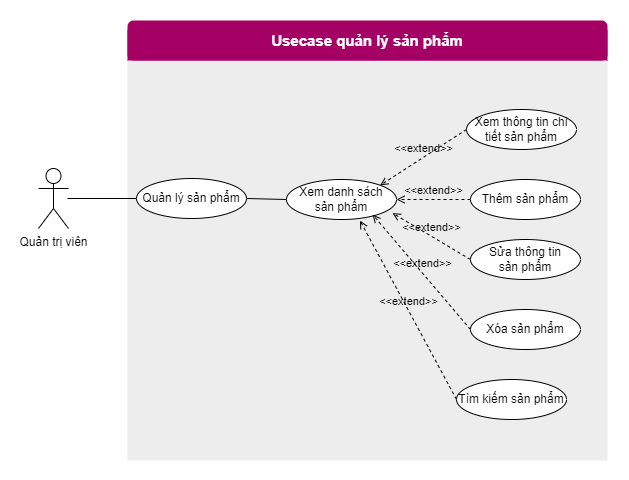
\includegraphics[width=15cm]{Images/usecase/ManageProduct.png}
            \caption{Use case diagram cho quản lý sản phẩm}
        \end{figure}
    \newpage
    \item \textbf{Mô tả usecase}
    \begin{longtable}{|p{3.5cm}|p{11.5cm}|}
        \hline
        Name &
          Xem thông tin chi tiết của sản phẩm \\ \hline
        Actor(s) &
          Quản trị viên \\ \hline
        Description &
          Cho phép quản trị viên xem thông tin chi tiết của tất cả các sản phẩm trên hệ thống \\ \hline
        Trigger &
          Quản trị viên chọn nút "Quản lý sản phẩm" tại trang giao diện chính của hệ thống\\ \hline
        Pre-condition(s) & \begin{tabular}[c]{@{}p{\linewidth}}
            - Quản trị viên đã đăng nhập vào hệ thống bằng tài khoản Manager\\
        \end{tabular} \\ 
          \hline
        Post-condition(s) &Quản trị viên xem được danh sách tất cả các sản phẩm trong hệ thống.\\ \hline
        
        Main Flow &
          \begin{tabular}[c]{@{}p{\linewidth}}
            1 . Hệ thống hiển thị danh sách tất cả các sản phẩm\\
        2 . Quản trị viên chọn cụ thể một sản phẩm bằng cách nhấn vào nút icon xem chi tiết\\
        3 . Hệ thống hiển thị thông tin chi tiết của sản phẩm\\
        \end{tabular} \\ \hline
        Alternative Flow &
          \begin{tabular}[c]{@{}p{\linewidth}} 
          \textbf{A1: Tại bước 1: }\\
         1.1. Quản trị viên nhấn tìm kiếm tên 1 sản phẩm cụ thể\\
        1.2.Hệ thống trả về các sản phẩm thỏa mãn tiêu chí tìm kiếm 
        \\
           
        \end{tabular} \\ \hline
          
        Exception & \begin{tabular}[c]{@{}p{\linewidth}} 
          None
        \end{tabular} \\ \hline
        \caption{Use-case xem thông tin chi tiết của sản phẩm}
    \end{longtable}
    \newpage
    
    \begin{longtable}{|p{3.5cm}|p{11.5cm}|}
        \hline
        Name &
          Quản lý sản phẩm - Thêm sản phẩm mới \\ \hline
        Actor(s) &
          Quản trị viên \\ \hline
        Description &
          Cho phép quản trị viên thêm một sản phẩm mới\\ \hline
        
        Trigger &
          Quản trị viên nhấn vào thêm sản phẩm\\ \hline
        
        Pre-condition(s) &
          \begin{tabular}[c]{@{}p{\linewidth}}
        Quản trị viên đã đăng nhập vào tài khoản của mình\\
        Quản trị viên đang trong màn hình quản lý sản phẩm\\
        
        \end{tabular} \\ \hline
          
        Post-condition(s) & Quản trị viên thêm sản phẩm thành công\\ \hline
        
        Main Flow &
          \begin{tabular}[c]{@{}p{\linewidth}}
        1 . Hệ thống chuyển sang giao diện nhập thông tin cho sản phẩm mới\\
        2 . Quản trị viên nhập lần lượt các thông tin mà hệ thống yêu cầu (tên sản phẩm, thể loại, giá bán, mô tả, ...)\\
        3 . Quản trị viên nhấn "Xác nhận" để thoát khỏi giao diện thêm sản phẩm\\
        4 . Hệ thống xác nhận thêm sản phẩm thành công\\
        \end{tabular} \\ \hline
        Alternative Flow &
          none \\ \hline
        Exception & \begin{tabular}[c]{@{}p{\linewidth}} 
        \textbf{E1: Tại bước 3:}\\
        - Hệ thống hiển thị lỗi "Tên/giá bán/... không hợp lệ"\\
        - Hệ thống hiển thị lỗi "Không được để trống thông tin"\\
        \end{tabular} \\ \hline
        \caption{Use-case thêm sản phẩm}
    \end{longtable}
    
    \begin{longtable}{|p{3.5cm}|p{11.5cm}|}
        \hline
        Name &
          Quản lý sản phẩm – Tìm kiếm sản phẩm\\ \hline
        Actor(s) &
          Quản trị viên \\ \hline
        Description &
          Cho phép quản trị viên tìm kiếm sản phẩm\\ \hline
        Trigger &
          \begin{tabular}[c]{@{}p{\linewidth}} 
        Quản trị viên nhấn vào ô tìm kiếm sản phẩm\\
        \end{tabular} \\ \hline
        Pre-condition(s) & \begin{tabular}[c]{@{}p{\linewidth}} 
        Quản trị viên đã đăng nhập vào tài khoản của mình\\
        Quản trị viên đang trong màn hình quản lý sản phẩm\\
        \end{tabular}\\
          \hline
        Post-condition(s) & Quản trị viên xem được thông tin sản phẩm đã tìm kiếm\\ \hline
        Main Flow &
          \begin{tabular}[c]{@{}p{\linewidth}}
        1 . Quản trị viên nhập từ khóa tên của sản phẩm cần tìm, rồi nhấn tìm kiếm\\
        2 . Hệ thống trả về danh sách tất cả sản phẩm thỏa mãn yêu cầu của từ khóa \\
        \\
        \end{tabular} \\ \hline
        Alternative Flow & None
         \\ \hline
        Exception & \begin{tabular}[c]{@{}p{\linewidth}} 
        \textbf{E1: Tại bước 2:}\\
        - Hệ thống hiển thị lỗi "Không có sản phẩm thỏa mãn yêu cầu"\\
        \end{tabular} \\ \hline
        \caption{Use-case tìm kiếm sản phẩm}
    \end{longtable}
    \newpage
    
    \begin{longtable}{|p{3.5cm}|p{11.5cm}|}
        \hline
        Name & Chỉnh sửa thông tin sản phẩm\\ \hline
        Actor(s) &
          Quản trị viên \\ \hline
        Description &
          Cho phép quản trị viên thay đổi thông tin sản phẩm trên hệ thống\\ \hline
        Trigger &
          Quản trị viên nhấn vào "Thay đổi thông tin sản phẩm" \\ \hline
        Pre-condition(s) & \begin{tabular}[c]{@{}p{\linewidth}} 
        Quản trị viên đã đăng nhập vào tài khoản của mình\\
        Quản trị viên đang trong màn hình quản lý sản phẩm\\
        Quản trị viên đã chọn được sản phẩm cần thay đổi thông tin\\
        \end{tabular}\\
        \hline
          
        Post-condition(s) & Quản trị viên đã thay đổi thông tin thành công cho sản phẩm\\ \hline
        
        Main Flow &
          \begin{tabular}[c]{@{}p{\linewidth}}
        1 . Hệ thống hiển thị 1 màn hình để chỉnh sửa các thông tin cần cho sản phẩm\\
        2 . Quản trị viên chỉnh sửa lần lượt các thông tin của sản phẩm
        3 . Quản trị viên nhấn "Cập nhật" để thoát khỏi giao diện chỉnh sửa thông tin sản phẩm\\
        4 . Hệ thống xác nhận chỉnh sửa thông tin sản phẩm thành công\\
        \end{tabular} \\ \hline
        Alternative Flow &
          None \\ \hline
        Exception & None \\ \hline
        \caption{Use-case chỉnh sửa thông tin sản phẩm}
    \end{longtable}
    
    \begin{longtable}{|p{3.5cm}|p{11.5cm}|}
        \hline
        Name & Xóa sản phẩm\\ \hline
        Actor(s) &
         Quản trị viên\\ \hline
        Description &
          Cho phép quản trị viên xóa sản phẩm khỏi hệ thống\\ \hline
        
        Trigger &
          Quản trị viên nhấn vào "Xóa sản phẩm" \\ \hline
        Pre-condition(s) & \begin{tabular}[c]{@{}p{\linewidth}} 
        Quản trị viên đã đăng nhập vào tài khoản của mình\\
        Quản trị viên đang trong màn hình quản lý sản phẩm\\
        B.M. đã chọn được sản phẩm muốn xóa\\   
        \end{tabular}\\
        \hline
          
        Post-condition(s) & Quản trị viên xóa thành công sản phẩm khỏi hệ thống\\ \hline
        
        Main Flow &
          \begin{tabular}[c]{@{}p{\linewidth}}
        1 . Hệ thống hiển thị 1 cảnh báo yêu cầu xác nhận xóa sản phẩm\\
        2 . Quản trị viên nhấn "Xác nhận xóa"\\
        3 . Hệ thống xác nhận xóa sản phẩm thành công\\
        4 . Quản trị viên nhấn "Xác nhận" để thoát khỏi giao diện xóa sản phẩm và trở về giao diện quản lý sản phẩm
        \\
        \end{tabular} \\ \hline
        Alternative Flow & None\\ \hline 
        Exception & None \\ \hline
        \caption{Use-case xóa sản phẩm}
    \end{longtable}
\end{enumerate}


\newpage
\subsubsection{Quản lý đơn hàng (admin)}
\begin{enumerate}[a. ]
    \item \textbf{Use-case diagram}
    \begin{figure}[h]
        \centering
        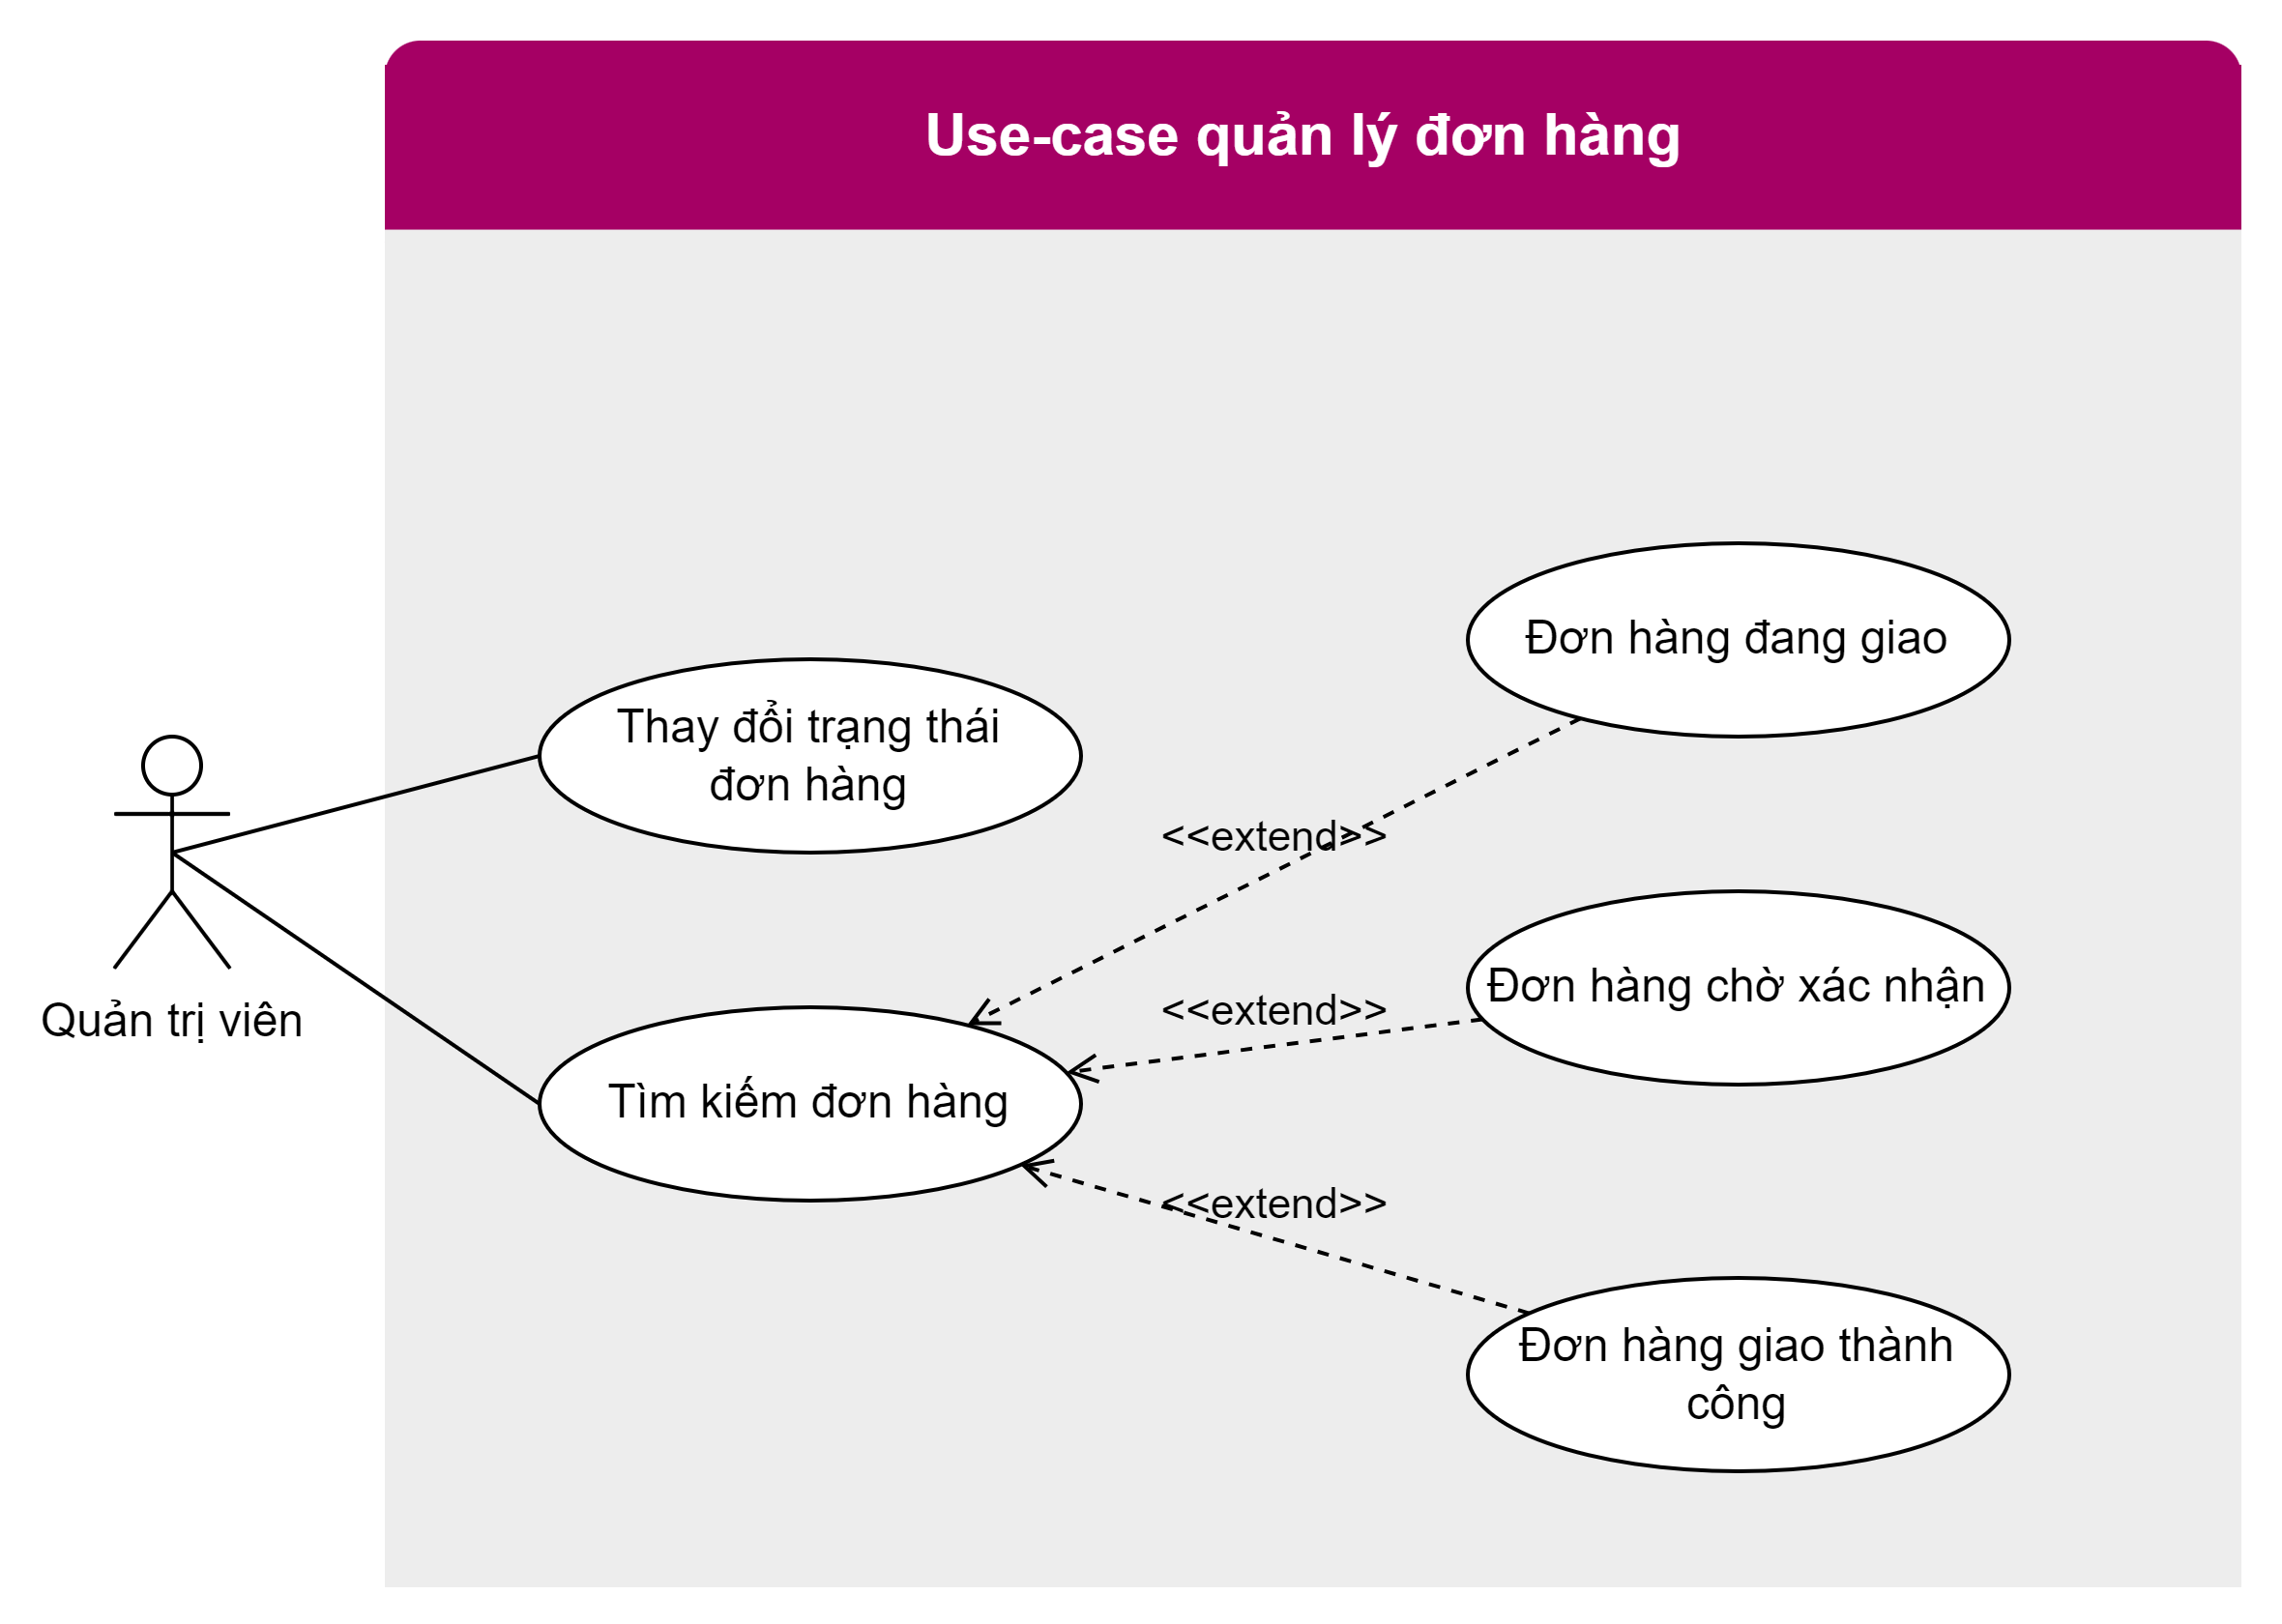
\includegraphics[width=10cm]{Images/usecase/use-case-manager-order.png}
        \newline
        \caption{Use-case diagram quản lý đơn hàng}
        \label{fig:enter-label}
    \end{figure}
    \item \textbf{Mô tả use-case}
    \begin{longtable}{|p{3.5cm}|p{11.5cm}|}
        \hline
        Name & Cập nhập trạng thái đơn hàng\\ \hline
        Actor(s) &
         Quản trị viên\\ \hline
        Description &
          Dùng để thay đổi trạng thái các đơn hàng như xác nhận để chuyển sang đang giao hàng và cuối cùng là giao hàng thành công\\ \hline
        
        Trigger & Cập nhập trạng thái đơn hàng \\ \hline
        Pre-condition(s) & \begin{tabular}[c]{@{}p{\linewidth}} 
        Quản trị viên đã đăng nhập vào tài khoản của mình \\
        Quản trị viên đang trong màn hình quản lý đơn hàng \\   
        \end{tabular}\\
        \hline
          
        Post-condition(s) & Cập nhập được trạng thái đơn hàng thành công\\ \hline
        Main Flow &
          \begin{tabular}[c]{@{}p{\linewidth}}
        1. Quản trị viên cần xác định đơn hàng cần thay đổi trạng thái \\
        2. Quản trị viên nhấn vào trạng thái đơn hàng và thay đổi \\
        3. Hệ thống hiện thông báo xác nhận thay đổi trạng thái đơn hàng\\
        4. Quản trị viên nhấn "Xác nhận" để thay đổi trạng thái đơn hàng.
        \\
        \end{tabular} \\ \hline
        Alternative Flow & None\\ \hline 
        Exception & None \\ \hline
        \caption{Use-case thay đổi trạng thái đơn hàng}
    \end{longtable}
\end{enumerate}
\subsection{Một số bài toán và giải pháp}
\subsubsection{Hệ thống gợi ý mua hàng}
\begin{enumerate}[a.]
\item \textbf{Khái niệm}\\
Hệ thống gợi ý mua hàng là một phần mềm hoặc công nghệ được sử dụng để cung cấp gợi ý và đề xuất sản phẩm cho người dùng dựa trên hành vi mua hàng trước đó, sở thích cá nhân, thông tin hồ sơ khách hàng, và các dữ liệu khác. Mục đích chính của hệ thống gợi ý mua hàng là cung cấp trải nghiệm mua hàng cá nhân hóa, tăng khả năng tương tác và mua hàng của khách hàng, và tăng doanh số bán hàng cho các doanh nghiệp.
\item \textbf{Các phương pháp hiện có}\\
Các hệ thống gợi ý mua hàng thường sử dụng các phương pháp và thuật toán khác nhau để đưa ra gợi ý sản phẩm. Dưới đây là một số phương pháp phổ biến:
\begin{itemize}
    \item \textbf{Gợi ý dựa trên sở thích cá nhân:} Hệ thống phân tích và đánh giá sở thích cá nhân của người dùng dựa trên lịch sử mua hàng, đánh giá sản phẩm, hoặc thông tin cá nhân khác để đề xuất các sản phẩm phù hợp.
    \item \textbf{Gợi ý dựa trên hành vi mua hàng tương tự:} Hệ thống phân tích hành vi mua hàng của người dùng và tìm kiếm những người dùng có hành vi mua hàng tương tự để đề xuất các sản phẩm mà họ có thể quan tâm.
    \item \textbf{Gợi ý dựa trên phân tích nội dung:}  Hệ thống phân tích nội dung sản phẩm, ví dụ: mô tả sản phẩm, danh mục, hoặc nguồn gốc, để đề xuất các sản phẩm tương tự hoặc liên quan.
    \item \textbf{Gợi ý dựa trên gom cụm (clustering): }Hệ thống phân tích và nhóm các sản phẩm vào các nhóm tương tự nhau và đề xuất các sản phẩm từ cùng một nhóm hoặc nhóm liên quan.
    \item \textbf{Gợi ý dựa trên kết hợp nhiều phương pháp:} Hệ thống kết hợp nhiều phương pháp và thuật toán để đưa ra gợi ý mua hàng chính xác và đa dạng.
\end{itemize}
\item \textbf{Hiện thực}\\
Trong nghiên cứu này, chúng tôi đã áp dụng công nghệ đồ thị của Neo4j vào hệ thống gợi ý mua hàng thông minh. Neo4j, một hệ quản trị cơ sở dữ liệu đồ thị phổ biến, cho phép chúng tôi lưu trữ và truy vấn dữ liệu có tính chất mối quan hệ phức tạp, như mối quan hệ giữa khách hàng, sản phẩm và các yếu tố khác.

Trước tiên, chúng tôi đã mô hình hóa thông tin về khách hàng bằng cách tạo các node đại diện cho khách hàng trong Neo4j. Mỗi node chứa các thuộc tính như sở thích cá nhân, lịch sử mua hàng, đánh giá sản phẩm và các thông tin cá nhân khác. Điều này giúp chúng tôi hiểu rõ hơn về sở thích và nhu cầu của từng khách hàng.

Tiếp theo, chúng tôi đã mô hình hóa các sản phẩm bằng cách tạo các node đại diện cho chúng trong Neo4j.
\begin{itemize}
    \item Product(id)
    \item User(id, phone\_number)
    \item Category(id)
\end{itemize}
Chúng tôi đã tạo các mối quan hệ giữa các sản phẩm dựa trên sự tương tự hoặc sự liên quan, cho phép chúng tôi tìm ra các mẫu và xu hướng trong dữ liệu sản phẩm. 
\begin{itemize}
    \item ADD\_TO\_WISH\_LISH(add\_at): Đây là mối quan hệ giữa User và Product. Mô tả cho việc User thêm sản phẩm vào mục yêu thích.

    \item BOUGHT(bought\_at): Đây là mối quan hệ giữa User và Product. Thể hiện việc khách hàng đã mua sản phẩm này.

    \item VIEWED(viewed\_at): Đây là mối quan hệ giữa User và Product. Thể hiện việc khách hàng đã ấn vào xem chi tiết sản phẩm.

    \item ADD\_TO\_CART(add\_at, variant\_id, quantity): Đây là mối quan hệ giữa User và Product. Thể hiện khách hàng đã thêm một sản phẩm vào giỏ hàng. Đây sẽ là nơi lưu giỏ hàng của khách hàng. Nhằm đảm bảo việc khách hàng dùng nhiều điện thoại thì giỏ hàng vẫn sẽ đồng bộ trên nhiều thiết bị.

    \item IS\_IN: Đây là mối quan hệ giữa Product và Category. Thể hiện việc product này thuộc về category nào
\end{itemize}
Chúng tôi đã sử dụng Neo4j để tạo các mối quan hệ giữa khách hàng và sản phẩm. Ví dụ, chúng tôi đã tạo mối quan hệ "BOUGHT" giữa khách hàng và các sản phẩm đã mua, cũng như mối quan hệ "VIEWED" giữa khách hàng và các sản phẩm đã xem. Điều này cho phép chúng tôi theo dõi hành vi mua hàng và gợi ý các sản phẩm phù hợp dựa trên sở thích và hành vi của khách hàng.

Để đề xuất các sản phẩm gợi ý, chúng tôi đã sử dụng truy vấn Neo4j để tìm kiếm các sản phẩm phù hợp. Ngoài ra chúng tôi sẽ sắp xếp dựa theo ngày mua của những sản phẩm để lấy ra sản phẩm cần gợi ý để tránh trường hợp sản phẩm khách hàng đã mua khá lâu còn gợi ý. Sau đây là một số phương pháp gợi ý mà chúng tôi sẽ áp dụng vào dự án.

\textbf{Gợi ý sản phẩm dựa trên những hành vi mua hàng tương tự nhau}

Phương pháp này phân tích bằng việc người dùng A và B có điểm chung gì trong việc mua hàng, xem sản phẩm và thêm vào yêu thích. Đầu tiên là A và B cùng mua 1 sản phẩm là Y và B cũng có mua thêm sản phẩm Z, thì lúc này hệ thống sẽ tính toán và trả về Z là sản phẩm cần gợi ý đến A.

Đầu tiên chúng tôi thực hiện lấy ra những sản phẩm dựa trên câu lệnh trên neo4j và sẽ nhận được kết quả là 1 danh sách các sản phẩm được gợi ý. Sau đó thực hiện lấy những sản phẩm đó từ trong database trả về cho người dùng.

\textbf{Gợi ý sản phẩm dựa trên những sản phẩm đã xem}

Đầu tiên chúng tôi sẽ lấy những sản phẩm mà khách hàng đã xem từ trong database được sắp xếp theo thời gian xem.

Sau đó chúng tôi sẽ lấy lần lượt những category trong sản phẩm. Bởi vì một sản phẩm có thể có nhiều category nên chúng tôi sẽ kiểm tra dựa trên những sản phẩm phải bao gồm luôn cả category trong sản phẩm đã mua đó. Nó sẽ trả về một danh sách của những category của sản phẩmVí dụ: sản phẩm A có category X1 và X2, sản phẩm B có Category là X3, X4 lúc này chúng ta sẽ trả về những danh sách category để thực hiện tìm kiếm: [[X1, X2], [X3, X4]]. Có nghĩa là ta sẽ lấy ra những sản phẩm có cùng category (điều kiện hợp) trong từng danh sách trên (điều kiện giao).

Thực hiện query những sản phẩm có category rồi trả về giao diện bán hàng.

\end{enumerate}
Bằng cách sử dụng Neo4j, chúng tôi đã tận dụng được tính năng mạnh mẽ của công nghệ đồ thị để lưu trữ và truy vấn dữ liệu một cách hiệu quả. Chúng tôi đã sử dụng ngôn ngữ truy vấn Cypher của Neo4j để tạo và truy vấn các node, mối quan hệ và thuộc tính trong hệ thống gợi ý mua hàng. Điều này đã giúp chúng tôi xây dựng một hệ thống gợi ý mua hàng thông minh hiệu quả và tốt
% \subsubsection{Hệ thống phân loại sản phẩm theo xu hướng thời trang}
\subsubsection{Hệ thống thanh toán}
\textbf{Cổng thanh toán PayOS}

Trong dự án này chúng tôi sử dụng thanh toán bằng hình thức chuyển khoản ngân hàng thông qua cổng thanh toán PayOS. Đây là cổng thanh toán thông qua VietQrPro. Ưu điểm của việc sử dụng cổng thanh toán này là không cần phải là doanh nghiệp thì mới có thể tích hợp cổng thanh toán mà chúng ta có thể tạo cổng thanh toán khi mà ta có thẻ ngân hàng và căn cước công dân.

Ngoài ra cổng thanh toán này còn hỡ trợ kiểm tra giao dịch real time (bắn Webhook về cho hệ thống chúng tôi). Sau đó chúng tôi sẽ dùng socket io để bắn giao dịch thành công đến ứng dụng khách hàng. Điều này sẽ làm cho việc mua hàng và thanh toán của người dùng mượt mà hơn, khi người dùng thanh toán thành công trên thiết bị của mình thì thông tin trạng thái thanh toán đơn hàng sẽ được tự động cập nhập.

\noindent Luồng thực thi của cổng PayOS

Sau khi người người dùng bâm thanh toán, sẽ chuyển người dùng đến trang thanh toán, đồng thời tạo một kết nối đến hệ thống để hệ thống có thể bắn message về ứng dụng khi đơn hàng thanh toán thành công.

Ở trên ứng dụng, khi người dùng đã thanh toán đơn hàng thành công thì lúc này hệ thống sẽ được PayOS gọi đế một API đã được định nghĩa sẵn ở hệ thống để nhận thông tin thanh toán, sau đó hệ thống sẽ lưu vào cơ sở dữ liệu đồng thời bắn message thanh toán thành công đến ứng dụng.
\begin{figure}[H]
    \centering
    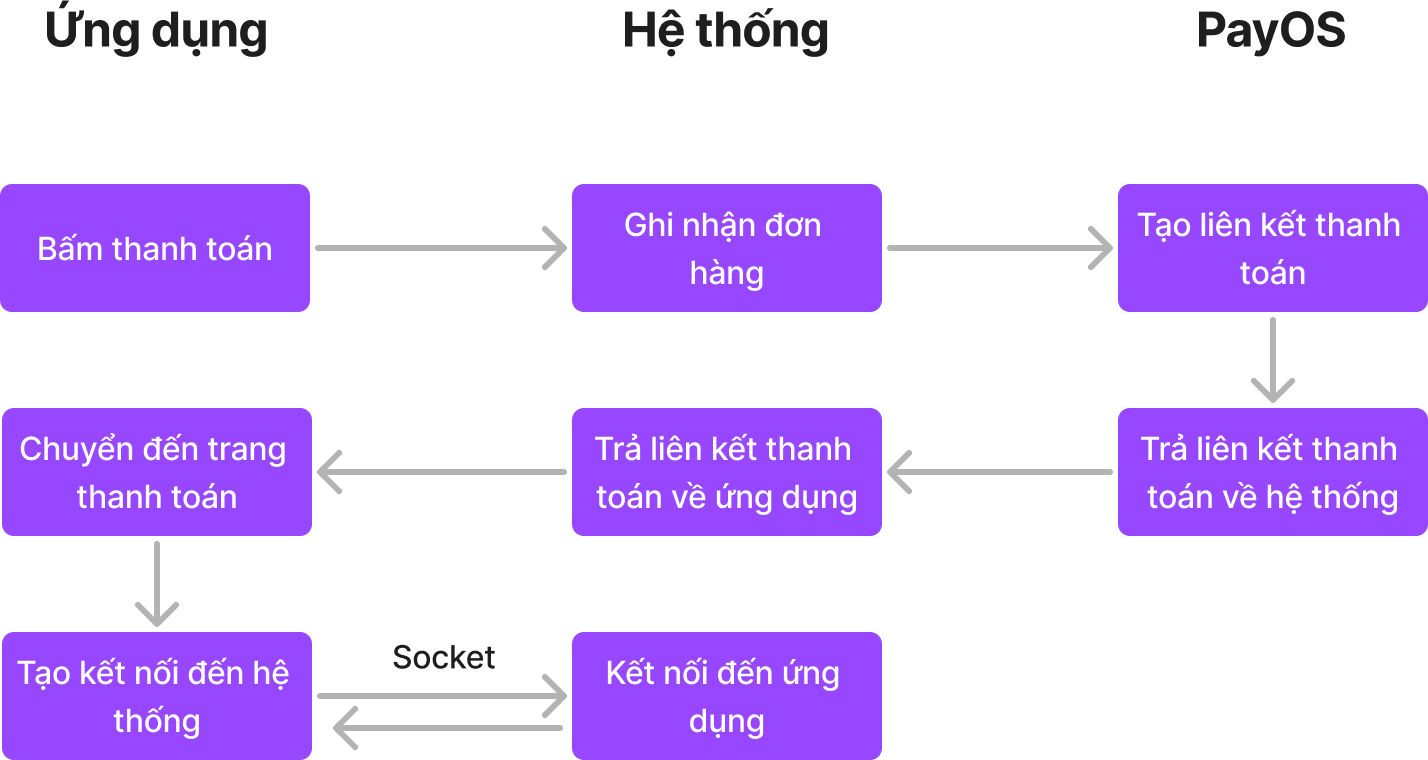
\includegraphics[width=15cm]{Images/payos-1.png}
    \newline
    \caption{Tạo connection đến ứng dụng}
    \label{fig:enter-label}
\end{figure}



\begin{figure}[H]
    \centering
    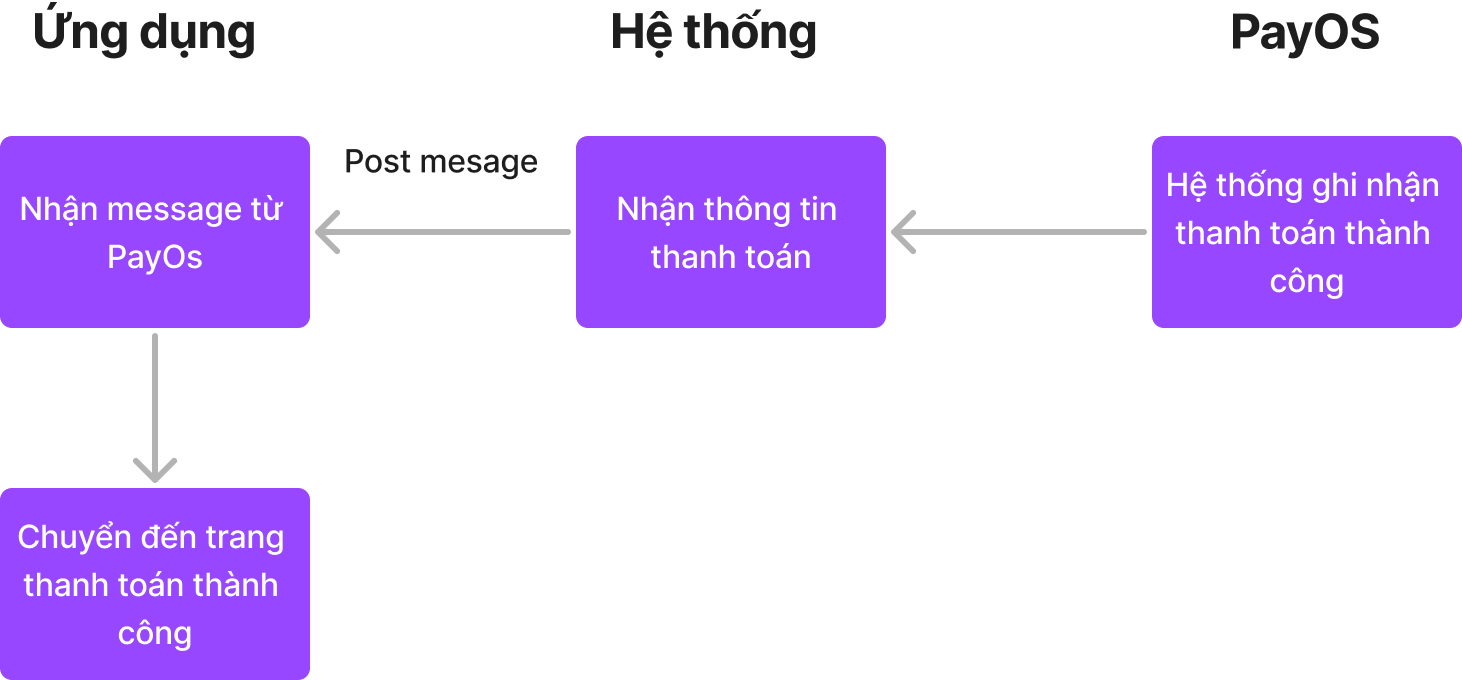
\includegraphics[width=15cm]{Images/payos-2.png}
    \newline
    \caption{Bắn message đến cho ứng dụng}
    \label{fig:enter-label}
\end{figure}

\subsubsection{Lọc và vô hiệu hóa các bình luận, đánh giá sản phẩm vi phạm tiêu chuẩn}
\begin{enumerate}[a.]
\item \textbf{Giới thiệu}\\
Mục tiêu là kiểm tra và loại bỏ các đánh giá/bình luận có chứa nội dung phản cảm dựa trên một số tiêu chí như chứa liên kết URL, sử dụng từ ngữ xấu, mức độ độc hại theo các tiêu chí như tấn công danh tính, xúc phạm, ngôn ngữ thô tục, độc hại nghiêm trọng, nội dung tình dục rõ ràng, đe dọa và độc hại.

\item \textbf{Mô tả giải thuật}\\
\textbf{Kiểm tra đường dẫn URL} \\
Sử dụng biểu thức chính quy (regular expression) để kiểm tra các đường dẫn URL, sau đó kiểm tra sự tồn tại của URL đó có chứa trong nội dung hay không. \\
\textbf{Kiểm tra từ ngữ xấu}\\
Sử dụng hàm badWords của thư viện vn-badwords để kiểm tra sự hiện diện của các từ ngữ cấm trong nội dung đánh giá sản phẩm. Hàm badWords sẽ kiểm tra nội dung có chứa các từ ngữ cấm hay không. Nếu có, hàm trả về true, ngụ ý rằng đánh giá sản phẩm sẽ bị vô hiệu hóa.\\
\textbf{Phân loại mức độ độc hại}\\
Sử dụng mô hình học sâu từ thư viện toxicity của Tensorflow: Hàm sử dụng mô hình này để phân loại nội dung dựa trên các tiêu chí độc hại. \\
Giá trị ngưỡng 0.9 được sử dụng để xác định độ nhạy của mô hình. Ngưỡng này có nghĩa là mô hình chỉ coi nội dung là phản cảm nếu độ tin cậy của kết quả phân loại cao hơn 90\%. Các nhãn (labels) mà mô hình này kiểm tra bao gồm: identity attack (tấn công danh tính), insult (xúc phạm), obscene (ngôn ngữ thô tục), severe toxicity (độc hại nghiêm trọng), sexual explicit (nội dung tình dục rõ ràng), threat (đe dọa) và toxicity (độc hại). Mô hình được tải với ngưỡng và các nhãn này để phân loại nội dung đánh giá sản phẩm.\\
Mô hình sẽ phân loại nội dung và trả về kết quả dưới dạng các nhãn với giá trị match (đúng hoặc sai) cho từng tiêu chí. Nếu bất kỳ nhãn nào xác định rằng nội dung là phản cảm (kết quả match là true), đánh giá sản phẩm sẽ bị đánh dấu là vi phạm tiêu chuẩn.
\end{enumerate}

\subsubsection{Tính năng tìm kiếm sản phẩm bằng hình ảnh}

\begin{enumerate}[a.]
\item \textbf{Khái niệm}\\
Tính năng tìm kiếm sản phẩm bằng hình ảnh là một công cụ mạnh mẽ và tiện ích trong các ứng dụng bán hàng trực tuyến, đặc biệt là ứng dụng bán quần áo. Tính năng này cho phép người dùng tải lên một bức ảnh của một sản phẩm (ví dụ như một chiếc áo sơ mi, một đôi giày, v.v.) và hệ thống sẽ tự động nhận diện và tìm kiếm các sản phẩm tương tự hoặc giống với sản phẩm trong bức ảnh đó trong cơ sở dữ liệu của cửa hàng.\\
\item \textbf{Mô tả giải thuật}


Tính năng này được xây dựng dựa trên phương pháp Content-based Image Retrieval (CBIR). Ảnh của các sản phẩm sau khi được lưu và ảnh của sản phẩm mà người dùng muốn tìm sẽ tiến hành trích xuất đặc trưng (feature extraction). \\
Trích xuất đặc trưng của ảnh (image feature extraction) là quá trình chuyển đổi hình ảnh từ dạng thô (các điểm ảnh) thành một vector đặc trưng (feature vector) mà máy tính có thể xử lý và hiểu. Chúng tôi sử dụng VGG16 model được tích hợp sẵn vào keras và được huấn luyện trước trên bộ dữ liệu ImageNet để thực hiện quá trình này.\\
Cấu hình mô hình: Tạo ra một hình con từ VGG16. Mô hình con này sẽ lấy đầu vào là hình ảnh và đầu ra là lớp fc1 của VGG16.\\
\textbf{Các bước trích xuất đặc trưng(feature extraction):}
\begin{enumerate}[1.]
    \item Mở hình ảnh từ buffer và chuyển đổi nó thành đối tượng PIL Image.
    \item Ảnh được chuyển sang dạng tensor trước khi đưa vào mô hình để trích xuất
    \item Đưa tensor vào mô hình tiến hành trích xuất đặc trưng. Nhận lại là một vector đặc trưng.
    \item Chuẩn hóa vector đặc trưng thành độ dài là 1. Điều này giúp thuận lợi trong quá trình so sánh vector sau này
\end{enumerate}
\textbf{Giải thuật Search by image:}
\begin{figure}[H]
    \centering
    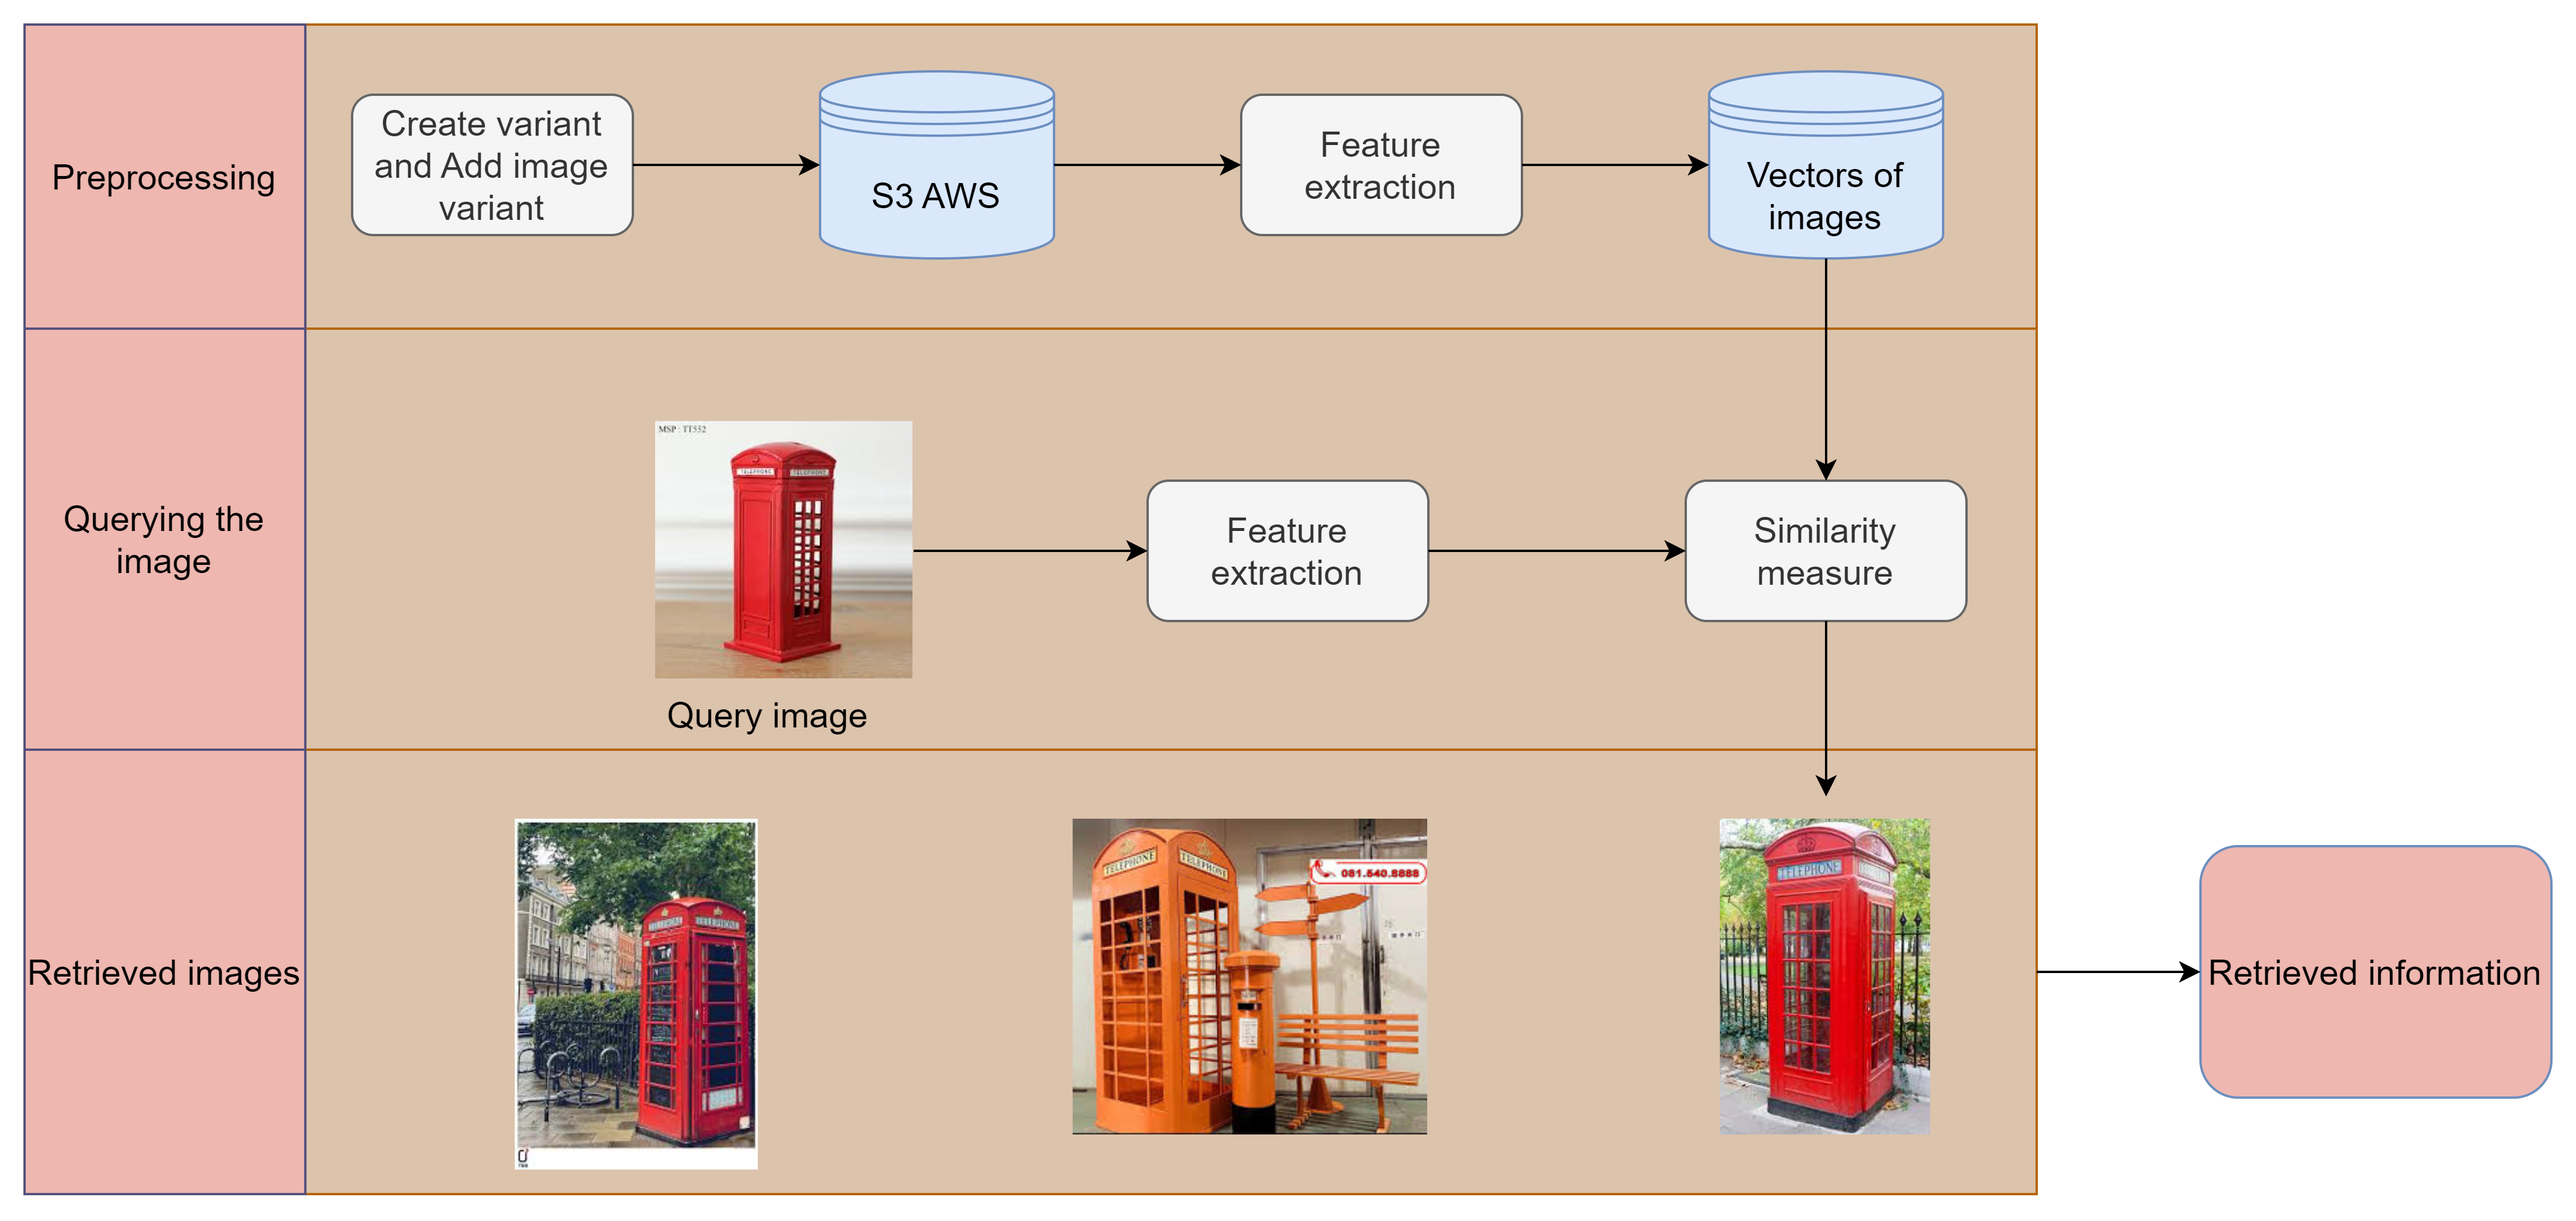
\includegraphics[width=15cm]{Images/search_by_image.png}
    \newline
    \caption{Giải thuật Search by image}
    % \label{fig:enter-label}
\end{figure}
\begin{enumerate}[1.]
    \item Preprocessing: Sau khi tạo variant và thêm ảnh lên S3 AWS. Các ảnh đó được tải lên và tiến hành trích xuất đặc trưng. Cuối cùng lưu vào kho chứa vector của ảnh.
    \item Querying the Image:  Người dùng cung cấp một hình ảnh truy vấn. Ảnh đó được tải lên và tiến hành trích xuất thành vector. Vector đó được đo khoảng cách với từng vector trong kho chứa vector bằng phương pháp tính khoảng cách Euclid. Từ đó, ta được danh sách các khoảng cách.

    \newpage
    \item Retrieved Images: Lấy ra các khoảng cách có giá trị thấp nhất, từ đó lấy được các ảnh và sản phẩm tương đồng với ảnh người dùng cung cấp
\end{enumerate}
\item \textbf{Hiện thực}\\
\noindent FastAPI là một framework hiện đại, nhanh chóng, và dễ sử dụng để phát triển các API với Python. Nó được xây dựng trên các công nghệ tiên tiến như ASGI (Asynchronous Server Gateway Interface) và sử dụng các thư viện mạnh mẽ như Starlette và Pydantic để cung cấp một trải nghiệm phát triển hiệu quả và mạnh mẽ.\\
Các ưu điểm của FastAPI:
\begin{itemize}
    \item Hiệu suất cao
    \item Dễ sử dụng
    \item Tài liệu tự động
    \item Xác thực và kiểm tra dữ liệu mạnh mẽ
    \item Hỗ trợ các tính năng hiện đại của Python
    \item Tích hợp dễ dàng với các thư viện khác
\end{itemize}
Vì các lý do trên, chúng tôi chọn xây dựng các API hỗ trợ cho tính năng Search by image bằng FastAPI.


\end{enumerate}








